\documentclass{report}

\usepackage{fancyhdr}
\usepackage{minitoc}
\usepackage{titlesec}
\usepackage{hyperref}
\usepackage{array}
\usepackage{titletoc}
\usepackage[table]{xcolor}
%\usepackage{tabularx}
\usepackage{ltablex}
\usepackage{ragged2e}
\usepackage{graphicx}
\usepackage{tikz}
\usepackage{aeguill}
\usepackage{amsmath}
\usepackage{mathtools}
\usepackage{enumitem}
\usepackage{caption}
\usepackage{etoc}

\makeatletter
\newif\ifTOC@marginpatched
\newcommand{\SetTOCrightmargin}[1]{%
\ifTOC@marginpatched\else
\let\old@pnumwidth\@pnumwidth
\let\old@dottedtocline\@dottedtocline
\def\@dottedtocline##1##2##3##4##5{%
    \old@dottedtocline{##1}{##2}{##3}{##4}{##5\hskip\TOC@rightmargin}}
\let\old@l@part\l@part
\def\l@part##1##2{\old@l@part{##1}{##2\hskip\TOC@rightmargin}}
\let\old@l@chapter\l@chapter
\def\l@chapter##1##2{\old@l@chapter{##1}{##2\hskip\TOC@rightmargin}}
\fi
\TOC@marginpatchedtrue
\edef\TOC@rightmargin{#1}%
\dimen0=\old@pnumwidth\relax
\advance\dimen0 by #1\relax
\edef\@pnumwidth{\the\dimen0}} %etoc style
\makeatother

\renewcommand{\listfigurename}{Table of all Found Issues}

% Copyright 2017 Sergei Tikhomirov, MIT License
% https://github.com/s-tikhomirov/solidity-latex-highlighting/

\usepackage{listings, xcolor}

\definecolor{verylightgray}{rgb}{.97,.97,.97}

\lstdefinelanguage{Solidity}{
	keywords=[1]{anonymous, assembly, assert, balance, break, call, callcode, case, catch, class, constant, continue, constructor, contract, debugger, default, delegatecall, delete, do, else, emit, event, experimental, export, external, false, finally, for, function, gas, if, implements, import, in, indexed, inline, instanceof, interface, internal, is, length, library, log0, log1, log2, log3, log4, memory, modifier, new, onBounce, optional, payable, pragma, private, protected, public, pure, push, repeat, require, responsible, return, returns, revert, selfdestruct, send, solidity, static, storage, struct, suicide, super, switch, then, this, throw, transfer, true, try, typeof, using, value, view, while, with, addmod, ecrecover, keccak256, mulmod, ripemd160, sha256, sha3}, % generic keywords including crypto operations
	keywordstyle=[1]\color{blue}\bfseries,
	keywords=[2]{address, bool, byte, bytes, bytes1, bytes2, bytes3, bytes4, bytes5, bytes6, bytes7, bytes8, bytes9, bytes10, bytes11, bytes12, bytes13, bytes14, bytes15, bytes16, bytes17, bytes18, bytes19, bytes20, bytes21, bytes22, bytes23, bytes24, bytes25, bytes26, bytes27, bytes28, bytes29, bytes30, bytes31, bytes32, enum, int, int8, int16, int24, int32, int40, int48, int56, int64, int72, int80, int88, int96, int104, int112, int120, int128, int136, int144, int152, int160, int168, int176, int184, int192, int200, int208, int216, int224, int232, int240, int248, int256, mapping, string, uint, uint8, uint16, uint24, uint32, uint40, uint48, uint56, uint64, uint72, uint80, uint88, uint96, uint104, uint112, uint120, uint128, uint136, uint144, uint152, uint160, uint168, uint176, uint184, uint192, uint200, uint208, uint216, uint224, uint232, uint240, uint248, uint256, var, void, ether, finney, szabo, wei, days, hours, minutes, seconds, weeks, years, ton, nanoton},	% types; money and time units
	keywordstyle=[2]\color{teal}\bfseries,
	keywords=[3]{block, blockhash, coinbase, difficulty, gaslimit, number, timestamp, msg, data, gas, sender, sig, value, now, tx, gasprice, origin},	% environment variables
	keywordstyle=[3]\color{violet}\bfseries,
	identifierstyle=\color{black},
	sensitive=false,
	comment=[l]{//},
	morecomment=[s]{/*}{*/},
	commentstyle=\color{gray}\ttfamily,
	stringstyle=\color{red}\ttfamily,
	morestring=[b]',
	morestring=[b]"
}

\lstset{
	language=Solidity,
	backgroundcolor=\color{verylightgray},
	extendedchars=true,
	basicstyle=\footnotesize\ttfamily,
	showstringspaces=false,
	showspaces=false,
	numbers=left,
	numberstyle=\footnotesize,
	numbersep=9pt,
	tabsize=2,
	breaklines=true,
	showtabs=false,
	captionpos=b
}



\newif\ifsolmodules
\newif\ifsoltables
\newif\ifsolissues
\newif\ifsoldraft

%\soldrafttrue
\soldraftfalse

%\solmodulestrue
\solmodulesfalse

\soltablestrue
%\soltablesfalse

%\solissuestrue
\solissuesfalse



\setcounter{secnumdepth}{4}
\setcounter{tocdepth}{4}

\titleformat{\paragraph}
{\normalfont\normalsize\bfseries}{\theparagraph}{1em}{}
\titlespacing*{\paragraph}
{0pt}{3.25ex plus 1ex minus .2ex}{1.5ex plus .2ex}

\newcommand\addcomment[3]{
  \addcontentsline{lof}{section}{#1}
  \noindent\begin{tabular}{|p{12cm}| }\hline
   \rowcolor{#2}{#1}\\
   {#3}\\\hline
  \end{tabular}
}

\newcommand\issueCritical[2]{\addcomment{\bf Critical issue: #1}{red}{#2}}
\newcommand\issueMajor[2]{\addcomment{\bf Major issue: #1}{pink}{#2}}
\newcommand\issueMinor[2]{\addcomment{\bf Minor issue: #1}{cyan}{#2}}

\ifsoldraft
\usepackage[firstpage]{draftwatermark}
\SetWatermarkText{Confidential}
\SetWatermarkScale{5}
\fi

\pagestyle{fancy}
\renewcommand{\footrulewidth}{0.4pt}
\fancyhead[RO,RE]{\leftmark}
\fancyhead[LO,LE]{\thepage}
\fancyfoot{}
\fancyfoot[RO,RE]{\thepage}
\fancyfoot[LO,LE]{\leftmark}

\pagestyle{fancy} % to have better page headers
\renewcommand{\headrulewidth}{2pt}
\fancyhf[lh,rh,ch]{}
\fancyhf[lh]{\begin{minipage}[b]{\textwidth}
        \begin{tabularx}{1\textwidth} { 
                >{\raggedright\arraybackslash}X 
                >{\raggedleft\arraybackslash}X 
            }
            \textit{\rightmark}&\textit{\leftmark}\\
        \end{tabularx}
    \end{minipage}}

\begin{document}

\title{Everscalend functional specification}
\author{By OCamlPro}
\maketitle
\dominitoc
\ifsolissues
\listoffigures
\fi
\tableofcontents


\etocsettocstyle{\subsection*{\contentsname}\hrule\smallskip
\begin{minipage}{.95\linewidth}}
{\end{minipage}\medskip\hrule} %etoc style

\ifsoldraft
\chapter{Only for Auditors}

\section{To edit this documents}

In the report.tex file, choose:
\begin{itemize}
\item{\bf \textbackslash{}soldraftfalse} to remove draft mode (watermarks, advises)
\item{\bf \textbackslash{}solmodulestrue} to display modules by chapter instead of contracts
\item{\bf \textbackslash{}soltablestrue} to display tables for parameters and returns
\item{\bf \textbackslash{}solissuesfalse} to remove the table of issues
\end{itemize}

Issues can be entered with:
\begin{itemize}
\item{\bf \textbackslash{}issueCritical\{title\}\{text\}}
\item{\bf \textbackslash{}issueMajor\{title\}\{text\}}
\item{\bf \textbackslash{}issueMinor\{title\}\{text\}}
\end{itemize}

\section{General Auditing Rules}

\begin{itemize}
\item Check that types have the correct integer types (Pubkey : uint256, \
   Amount: uint128, Time: uint64 ).
\item Naming conventions: constants should for example be all uppercase, static variables should start with a prefix like \verb+s_+, globals should start with a prefix like \verb+g_+ or \verb+m_+, internal functions should start with a prefix \verb+_+.
\item Numbers should not appear in source, but be defined as constants.
\item In constant definitions, verify that 2 consecutive errors have not the same error (common copy-paste error)
\item Constants for amounts should be expressed in \verb+ton+ to prevent too many zeroes.
\item Modifiers with {\tt tvm.accept} must always check the source of the message
\item Constructors with arguments must always check the source of the message to prevent anybody from calling the constructor and set variables instead of the real owner
\item Failures should never happen after {\tt tvm.accept} (such as {\tt require}, division by zero, overflows, etc.)
\item Most arguments should be protected by a {\tt require}
\item Before sending a message, the function should check that it has enough gas (to prevent a partial failure during the message sending phase)
\item {\tt tvm.accept} should only be called after verifying that the sender of the message if the contracts' owner
\end{itemize}
\fi

\chapter{Introduction}


This is a security audit of the ``...'' smart contract,
whose source code is available at
\url{https://github.com/...}, commit
\verb+...+. This security audit is provided as a submission to
Formal Method Sub-Governance Contest
\url{https://formet.gov.freeton.org/...}.

During this audit, we used the following classification of our findings, into three kinds of issues:
\begin{itemize}
\item {\bf Critical Issues:} such issues can lead to taking ownership of resources (tokens, contracts), or total
  disabling of the service;
\item {\bf Major Issues:} such issues can lead to a decrease in the quality of the service,
  or temporary loss of availability;
\item {\bf Minor Issues:} Such issues do not impact the service
  itself. For example, code improvements to improve readability, to
  improve sharing, etc.
\end{itemize}

We found XX critical issues, YY major issues and ZZ minor issues
during this audit of the contracts.

\begin{itemize}
\item {\bf XX Critical Issues:}
\item {\bf YY Major Issues:}
\item {\bf ZZ Minor Issues:}
\end{itemize}

For easier access to issues, we provided a table of issues at the
beginning of the document.



\chapter{High-level system description}


\section{System purpose}

Everscalend is a DEFI (DEcentralized FInance) lending and borrowing system implemented on the Everscale Blockchain. It's main purpose is to provide Everscale users with a realiable way to lend and borrow cryptocurrency tokens. It makes it possible for users to generate profits on tokens they supply for lending and to acquire tokens by borrowing them instead of buying them.

\section{Terms of the system domain}

\begin{tabularx}{\linewidth}{|l|X|}
  \hline
  \multicolumn{1}{|c|}{\textbf{Term}} & \multicolumn{1}{c|}{\textbf{Definition}} \\\hline
  \endhead

  Interest rate & The rate of profit that the lenders get when tokens are borrowed. The interest rates in Everscalend are algorithmically calculated and they increase when the borrowing demand increases and decrease when it does. \\\hline
  
  Reserve factor & Ranging from 0 to 1, it represents the portion of the interest rate that should be stored in the reserve whenever it is acquired. \\\hline
  
  Market & A pool of tokens of the same kind where all the tokens supplied by the users are stored. It also holds information like the exchange rate and reserve factor etc. \\\hline
  
  vToken & A virtual token, it is used to represent the amount of tokens that a supplier owes the market and they get them whenever they supply tokens to the markets. There is a type of vToken for each type of token. When interest rate accumulates on the supplied tokens in the markets, the exchange rate from the vTokens to the real tokens increases, so when a supplier holding vTokens wishes to withdraw. They will be able to withdraw more than they supplied, the difference representing the interest that was accumulated on their supplied tokens. \\\hline
  
  Collateral & The amount of vTokens that a borrower has to have in order to be able to borrow a certain amount of some tokens. \\\hline
  
  Collateral factor & Ranging from 0 to 1, it represents the amount of tokens that can be borrowed for a collateral. e.g. a collateral factor of 0.9 allows the borrowing of a number of tokens worth $90\%$ of the collateral. \\\hline
  
  Account health & A fraction of the sum of the USD value of a user's supplied tokens divided by the sum of the USD value of all the tokens they borrowed. It is used to determine whether a user is eligible for liquidation or not. When nominator is greater than the denominator in that fraction, we say that the user's account healthy, otherwise it is unhealthy. \\\hline
  
  Liquidation & The process in which some user's debt is liquidated by another user, by paying a portion of the owed tokens in exchange for the borrower's vTokens at a better exchange rate than the market. \\\hline
  
  Liquidation Multiplier & A value superior to 1. It is the amount by which the amount of vTokens that the liquidator should get by market price is multiplied to increase it. \\\hline

  Index & Refers to the interest rate index, which is a value that captures the history of interest rates of a market. It is updated after each transaction to compound the interest since the previous index. \\\hline
\end{tabularx}

\newpage
\section{Mathematical notations}
\label{spec:mn}
The following mathematical notations are used in the document to simplify the equations. They are to be considered whitin the context in which they are used.

\newcommand\USD{\mathit{USD}}

\newcommand\M[1]{\mathit{m_{#1}}}
\newcommand\T[1]{\mathit{T_{#1}}}

\newcommand\ER[2]{\mathit{ER(#1, #2)}}

\newcommand\BA[1]{\mathit{Ba(#1)}}
\newcommand\C[1]{\mathit{C(#1)}}

\newcommand\UR[1]{\mathit{UR_{#1}}}
\newcommand\UM[1]{\mathit{UM_{#1}}}
\newcommand\UBR[1]{\mathit{UbR_{#1}}}
\newcommand\BIR[1]{\mathit{BIR_{#1}}}
\newcommand\RF[1]{\mathit{RF_{#1}}}

\newcommand\RTB[1]{\mathit{rTB(#1)}}
\newcommand\VTB[1]{\mathit{vTB_{#1}}}
\newcommand\RES[1]{\mathit{Res_{#1}}}

\newcommand\CF[1]{\mathit{CF(#1)}}
\newcommand\AH[1]{\mathit{AH_{#1}}}
\newcommand\BC[1]{\mathit{BC_{#1}}}

\newcommand\IND[2]{\mathit{Ind_{#1, #2}}}
\newcommand\INDL[1]{\mathit{Indl_{#1}}}
\newcommand\AI[1]{\mathit{AI_{#1}}}

\begin{tabularx}{\linewidth}{|l X|}\hline
  $\M{T}$: & Market for tokens of type $T$ \\\hline
  $vT$: & the vToken type of token \\\hline
  
  $\ER{\T{1}}{\T{2}}$: & Exchange rate from the token $\T{1}$ to the token $\T{2}$, aka the $x$ in: $1\ \T{1} = (x \times 1)\ \T{2}$ \\\hline
  
  $\BA{m}$: & Borrowed amount of tokens in a market $m$ \\\hline
  $\C{m}$: & Amount of cash in a market $m$ \\\hline

  $\UR{m}$: & Utilization ratio of the market $m$ \\\hline
  $\UM{m}$: & Utilization multiplier of the market $m$ \\\hline
  $\UBR{m}$: & Utilization base rate of the market $m$ \\\hline
  $\BIR{m}$: & Borrowing interest rate of the market $m$ \\\hline
  $\RF{m}$: & Reserve factor of the market $m$ \\\hline

  $\RTB{m}$: & Real token balance of the market $m$ \\\hline 
  $\VTB{m}$: & vToken balance of the market $m$ \\\hline 
  $\RES{m}$: & Amount of tokens stored in the reserves of the market $m$ \\\hline
  
  $\CF{T}$: & Collateral factor for a token T \\\hline
  $\AH{u}$: & User's account health \\\hline
  $\BC{u}$: & User's borrowing capacity \\\hline
  
  $\IND{m}{n}$: & $n$th interest rate index of the market $m$ \\\hline
  $\INDL{m}$: & Latest interest rate index of the market $m$ \\\hline
  $\AI{m}$: & accumulated interest of the market $m$ \\\hline

\end{tabularx}
\newpage
\section{System functioning}

the Everscalend system uses markets, which are pools of tokens with algorithmically calculated interest rates, based on the supply and demand for the tokens they hold. Each market is unique to a cryptocurrency, and contains a transparent and publicly-inspectable ledger, with a record of all transactions and historical interest rates. 

The lenders and the borrowers of tokens interact directly with the system, earning and paying a variable interest rate, without having to negotiate terms such as the interest rate or the value of collateral with a peer or counterparty.

In this section we describe the functioning of the system.

\subsection{Kinds of users}

There are two kinds of clearly identifiable users:
\begin{itemize}
  \item The admin who is the deployer of (at least one of) the main contracts of the system like \verb|MarketAggregator|, \verb|WalletController| or \verb|Oracle|.
  \item The ``normal'' users who interact with the system. 
\end{itemize}
And there are four roles that can be taken by the users and which determine their permissions when it comes to interacting with the system:
\begin{itemize}
  \item Owner: this is the role of the admin only. It gives them the right to modify all the parameters of the system. 
  \item Upgrader: this role can be given to a user by the owner and it gives them the right to upgrades some contracts' codes.
  \item Parameter changer: this role can be given to a user by the owner and it gives them the to modify some of the parameters of the system.
  \item Other: this is the role of all the users who don't have a privileged role and can only interact with the system to realise the market opeartions (supply, borrow ...) without being able to manually change the parameters of the system. 
\end{itemize}

\subsection{User capabilities}

In this section we describe what (non-privileged) users can do by using the system. 

\subsubsection{Supply}

A user that wishes to make a certain amount of their tokens available for borrowing has to supply them to the system. The supplied tokens are then aggregated to the tokens of the same kind that were supplied by other users.

The supplier receives vTokens for their supply that they can use as collateral to borrow other tokens. vTokens are a currency used to represent how many of the real tokens in the market a user can withdraw, they also determine how many he can borrow of other tokens.

\subsubsection{Withdraw}

A user who owns vTokens can pay with them to withdraw the tokens he supplied. The user can do it at any time provided that their account is healthy, aka $\AH{u} > 1$ with $\AH{u}$ being the user $u$ account health

\subsubsection{Borrow}
To borrow a certain amount of some token:

\begin{itemize}
  \item There have to be enough tokens in the market for borrowing.
  \item The borrowed amount has to be within the user's borrowing capacity, noted $BC_u$ with $u$ being the user.
\end{itemize}

The user's $BC_u$ represents the amount of vTokens that the user can still use as collateral to borrow. Once that amount is reached, the user can no longer perform any action that costs them vTokens like borrowing or withdrawing.

\subsubsection{Repay}

A borrower can repay the amount they borrowed by returning it to the market. By doing that the collateral they set for the borrowing is freed and can be used to borrow other tokens.

\subsubsection{Liquidate}

When a user's account is unhealthy, aka ($AH_u < 1$), the liquidation of his debt becomes possible. The liquidation process consists of selling the borrower's collateral vTokens at a discount in exchange for the repayment of the borrower's debt or a portion of it.

The purpose of this mecanism is to financially incentivize the liquidators to add liquidity to the system and pay other users' debts.

\subsection{Key system algorithms}

\subsubsection{Interest acquisition}

The values of interest rates increase when the demand is high and decrease when it is low. The calculation of the real interest requires some intermediary variables:

\begin{itemize}
  \item The utilisation ratio $\UR{m}$ for a market $m$: 
  $$
    \UR{m} = \frac{ \BA{m} }{ \RTB{m} + \BA{m} }
  $$
  The utilisation ratio unifies supply and borrowing demand into a single variable and shows which markets are demand.
  \item The borrowing interest rate:
  $$
    \BIR{m} = \UR{m} * \UM{m} + \UBR{m}
  $$ % in: MarketOperations.calculateBorrowInterestRate
\end{itemize}
The accumulated interest can then be calculated as follows:
$$
  \AI{m} = \BA{m} \times \BIR{m} \times \Delta t
$$ % in: MarketsAggregator.finterestAccumulated
with $\Delta t$ being the time difference in seconds, between the current time and the last moment at which the interest rate was calculated.

\subsubsection{Interest rate indexes}

Each time the interest rate is calculated in a certain market, the interest rate index associated to that market is updated. New indexes are calculated as follows: 
$$
\IND{m}{n} = (\BIR{m} \times \Delta t + 1) \times\IND{m}{n-1}
$$
With $\IND{m}{0} = 1$.

\subsubsection{Reserves}

When interest is accumulated, a portion of it, the size of which is determined by the reserve factor, is put in a reserve, the rest of it is stored as cash. After accumulating the interest, the reserve is updated by adding $(\AI{m} \times \RF{m})$ to it.

The purpose of the reserves is to protect a portion of the lenders interest so that they don't lose everything in case of liquidation, only their cash can be liquidated. 

\subsubsection{vToken exchange rate calculation}

As stated previously the exchange rates from vTokens to real tokens depend on the supply and borrowing demand of those tokens. It is calculated as follows:

$$
\ER{vT}{T} = \frac{\RTB{\M{T}} + \BA{m} - \RES{\M{T}}}{\VTB{\M{T}}}
$$

\subsubsection{Account health and borrow capacity calculation}

A user $u$'s account health determines whether or not it is liquidable, if $AH_u < 1$ then it is otherwise it isn't. If the user's account is liquidable then the user can't withdraw their tokens or borrow more tokens before some other users liquidiates them or they supply more tokens to the market to improve their account's health. The account's health is calculated whenever the user tries to perform any market operation or gets one of his loans liquidated.

\noindent Given: 
$$
  sval(T, vTsa) = \frac{vTsa \times \ER{vT}{T}}{\ER{T}{\USD}} \times \CF{T}
$$
and
$$
  bval(\M{T}, ba, ind) =\begin{dcases}
    0 & ba = 0\\
    \frac{(ba \times ind)/ \INDL{\M{T}}}{\ER{T}{\USD}} & ba \neq 0 \wedge \INDL{\M{T}} \neq ind \\
    \frac{ba}{\ER{T}{\USD}} & ba \neq 0 \wedge \INDL{\M{T}} = ind
    \end{dcases}
$$
It is calculated as follows:
$$
  AH_u = 
    \frac { 
      \sum_{(T_i, vTsa) \in SI_u} 
        sval(T_i, vTsa)
    } { 
      \sum_{(\M{T_j}, ba, ind) \in BI_u} 
      bval(\M{T_j}, ba, ind)
    }
$$
Where: 
\begin{itemize}
  \item $SI_u$: The supply information of the user $u$, which consists of a collection of couples $(m_{T_i}, vTsa_i)$ with: 
  \begin{itemize}
    \item $T_i$: the kind of the supplied token;
    \item $vTsa_i$: the amount of vTokens that the user got from the supply. 
  \end{itemize}
  \item $BI_u$: The borrow information of the user $u$, which consists of a collection of triplets $(m_{T_j}, ba, ind)$ with: 
  \begin{itemize}
    \item $T_j$: the kind of the borrowed token;
    \item $ba$: the amount that was borrowed;
    \item $ind$: the value of the interest rate index when the borrowing occured. 
  \end{itemize}
\end{itemize}

A user's borrowing capacity is a value in USD that determines how many vTokens a user can use as collateral or redeem, the limit being that the vToken's worth has to be less that the user's borrowing capacity. The borrowing capacity is calculated as follows: 
$$
  BC = (\sum_{(m_{T_i}, vTsa) \in SI_u} sval(T_i, vTsa)) - (\sum_{(m_{T_j}, ba, ind) \in BI_u} bval(m_{T_j}, ba, ind))
$$

\subsubsection{Liquidation}

The amount of vTokens the liquidator gets is calculated thanks to the liquidation multiplier $LU$ which is the value by witch the amount of tokens they would get at market price is multiplied to increase it. If a liquidator wants to repay a portion $R_T$ of a borrower's debt in tokens of type $T$, the amount of the borrower's vTokens that the liquidator will get $vTA$ is calculated as follows:
$$
  vTA = R_T \times \ER{T}{vT} \times LU
$$
The value of the liqudation multiplier is set manually by the admin.

\subsubsection{Module locking mecanism (TODO)} 

To avoid messing up with the pools of tokens and market parameters while a user is performing an operation, a locking mecanism is used, that prevents the modification of the data that is used during the user's operation. The locks are especially necessary when try to extract tokens from the markets by borrowing or withdarwing, or from other users through liquidation 

Such locks are used in:
\begin{itemize}
  \item \verb|BorrowModule|: The lock prevents other users from borrowing at the same time.
  \item \verb|LiquidationModule|: In this case the lock is on the liquidated user, the purpose is to prevent more than one user liquidating the same user's debt. 
  \item \verb|WithdrawModule|: To prevent other users from withdrawing while one of them has started that process. 
  \item \verb|UserAccount|: This conract uses two locks called \verb|borrowLock| and \verb|liquidationLock|. As their names suggest, \verb|borrowLock| locks the user's account during the processing of a borrow request, stopping the user from doing another one before the current one is finished. The \verb|liquidationLock| stops the user from withdarwing or borrowing while he is being liquidated. 
\end{itemize}

\section{Architecture of the System}

\begin{figure}[h!]
  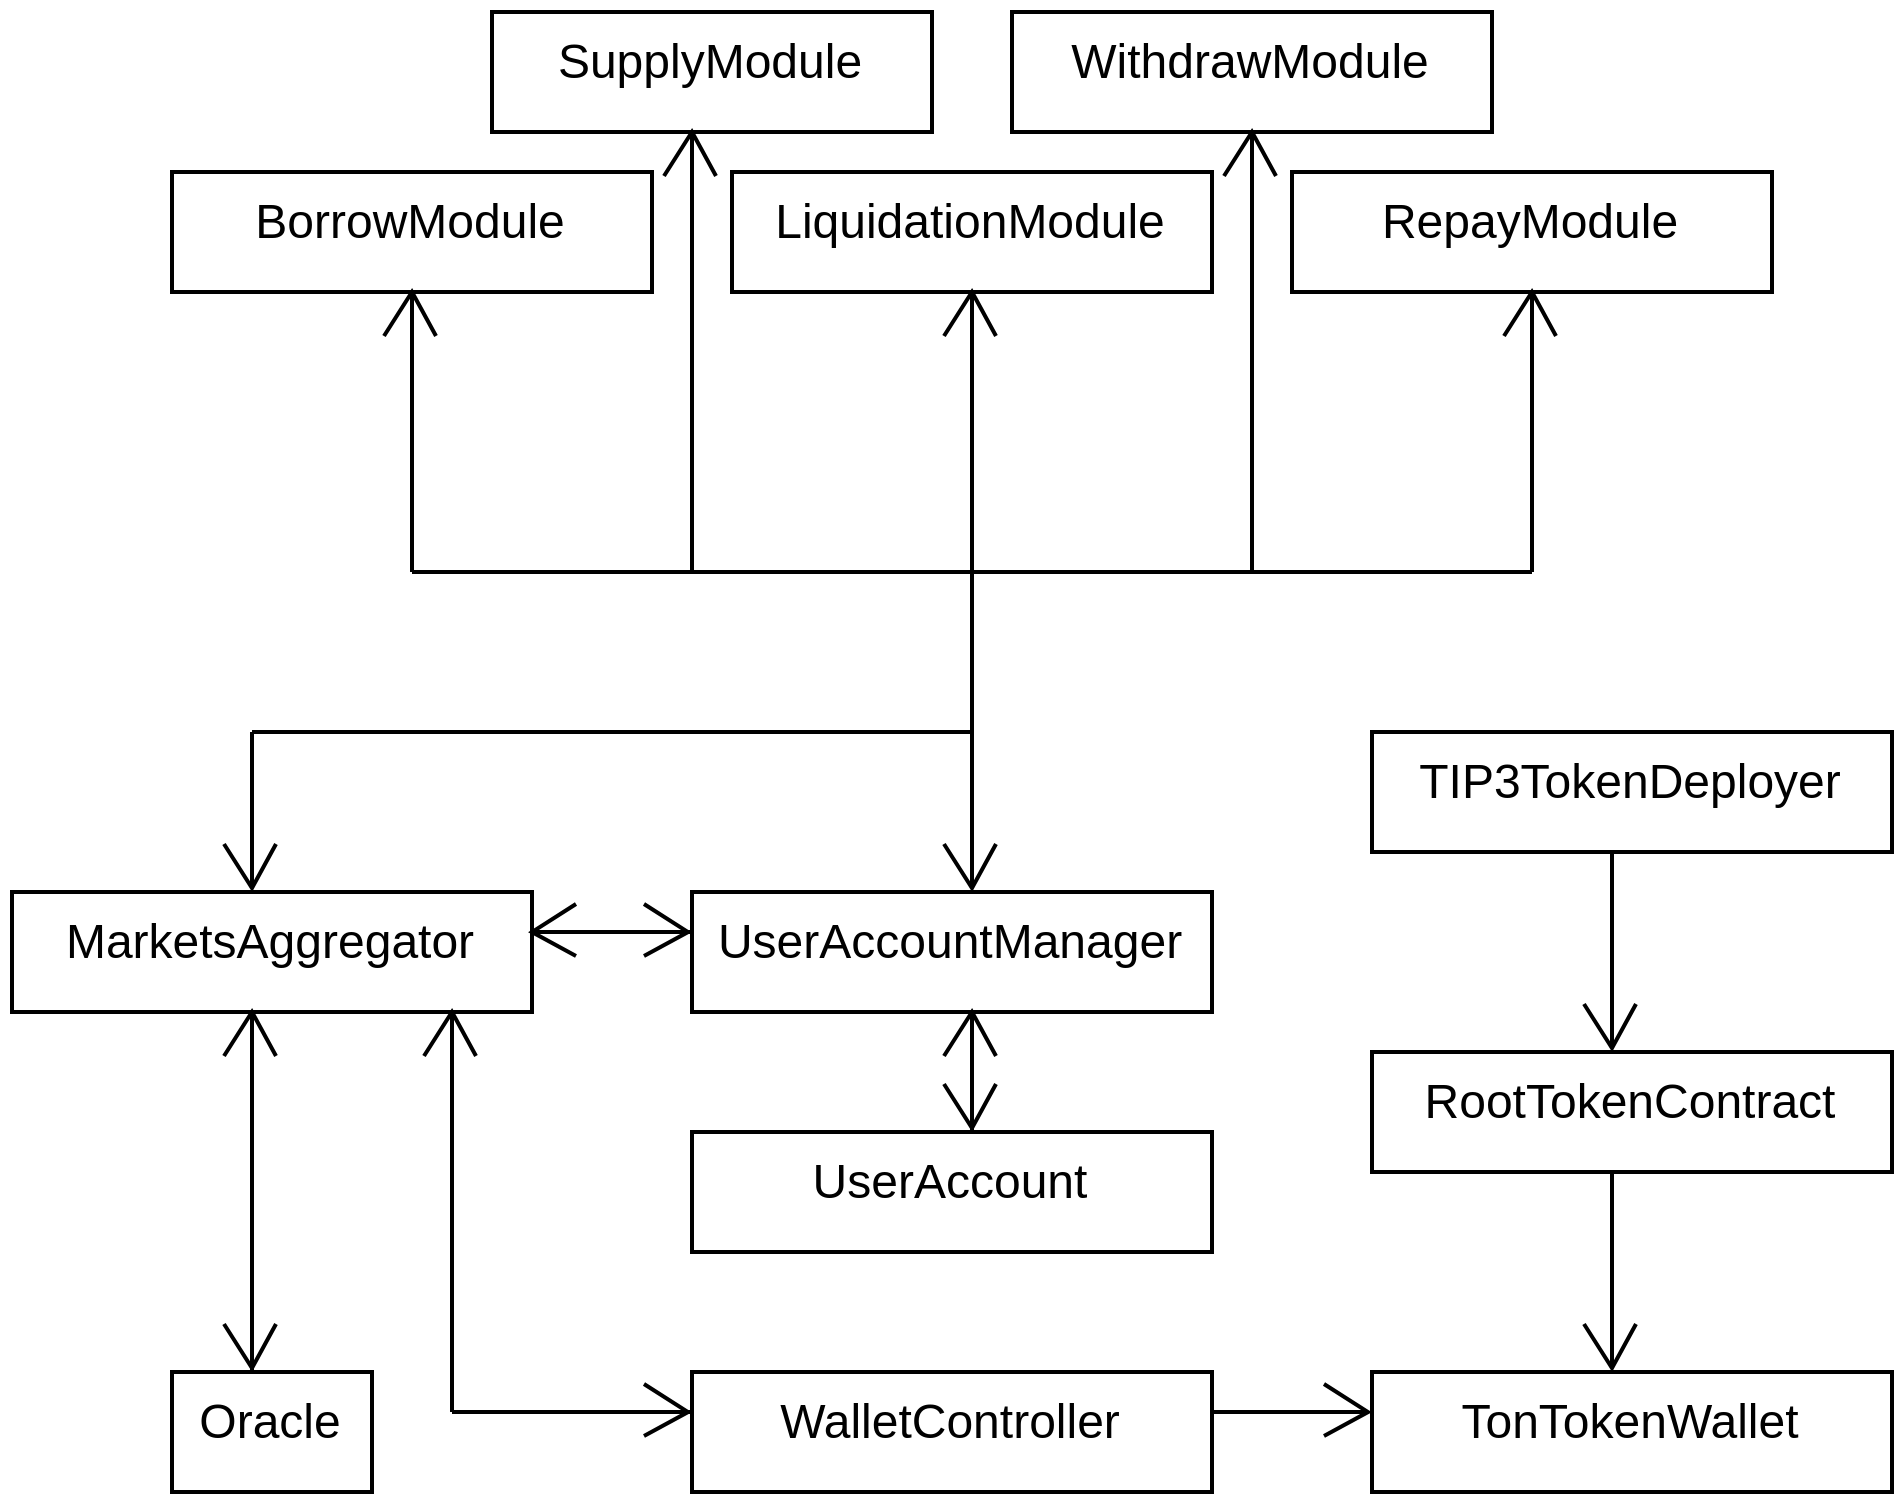
\includegraphics[width=\textwidth]{./assets/archi.png}
  \caption{System architecture with smart contract interactions}
  \label{fig:archi}
  \captionsetup[figure]{list=no} %So that it doesn't appear in list of figures
\end{figure}

Figure~\ref{fig:archi} shows a simplistic representation of the architecture of the system. The main smart contracts are shown with their names only while the interfaces, libraries and the smart contracts that are not necessary for comprehension were omitted. The smart contracts are connected with arrows which are meant to show interactions between them, these interactions will be described below.

\subsection{Main smart contracts}

\subsubsection{MarketsAggregator}

It mainly serves as a container for all the necessary information surrounding the markets, like the interest rates, the exchange rates and the borrow and supply amounts of each market.

\paragraph*{Functionalities:}
\begin{itemize}
  \item Adding and removing markets. 
  \item Updating the information on the markets. Either following market operations from users (like supplying, borrowing ... etc) or changes in the prices of the supported tokens. 
\end{itemize}

\paragraph*{Interactions:}
\begin{itemize}
  \item Oracle: to get token price updates.
  \item Operations modules: to perform market operations.
  \item UserAccountManager: to update account health after performing operations.
  \item WalletController: to transfer tokens to(from?) when necessary.
\end{itemize}

\subsubsection{Operations modules}

These smart contracts are used to help perform the market operations by doing the necessary math for these operations. 

\paragraph*{The smart contracts:}
\begin{itemize}
  \item SupplyModule
  \item WithdrawModule
  \item BorrowModule
  \item RepayModule
  \item LiquidationModule
\end{itemize}

\subsubsection{Oracle}

It is used by the MarketsAggregator smart contract to get price updates on the supported tokens in the markets.

\subsubsection{TonTokenWallet}

It serves as a TIP-3 token wallet and it handles token transfers to and from the wallet. Everscalend follows the TIP-3 token standard and these wallets are necessary to interact with the system. They can be delpoyed either by RootTokenContract or the a user who has the address of the RootTokenContract associated to the wallet's token.

\paragraph*{Functionalities:}
\begin{itemize}
  \item Tranfer tokens to and from the wallet.
  \item Deploy a receiver's TonTokenWallet and transfer tokens to it.
  \item Burn tokens.
\end{itemize}

\subsubsection{RootTokenContract}

A contract that is deployed by a token owner and stores information about the root token (like its name, symbol and total supply).

\paragraph*{Functionalities:}
\begin{itemize}
  \item Minting tokens.
  \item Deploying instances of TonTokenWallet.
  \item Updating the information on the root token.
  \item Change root token owner.
\end{itemize}

\subsubsection{TIP3TokenDeployer}

it deploys RootTokenContract contracts.

\subsubsection{WalletController}

It's the smart contract that controls all the TIP-3 wallets of the markets and managers the operations that require token transfers to and from those wallets.

\paragraph*{Functionalities:}
\begin{itemize}
  \item Adding and removing market wallets. 
  \item Getting information about market wallets. 
  \item Decodes the payloads of messages that require TIP-3 token transfers and adds necessary information like message origin and token amount before passing to MarketsAggregator.
  \item Allows user to perform the supply, repay and liquidate operations.
\end{itemize}

\paragraph*{Interactions:}
\begin{itemize}
  \item MarketsAggregator: to communicate to it the details of the market operations that require TIP-3 token transfer into the wallets of the markets.
  \item TonTokenWallet: to transfer tokens a user's wallet.
\end{itemize}

\subsubsection{UserAccount}

It's used to store information about how a user interacts with the markets, like how much they borrowed from which market and how much they supplied to which market. It also allows the user to perform the borrow and withdraw operations.

It interacts only with UserAccountManager, which can request the information and to which it returns it.

\subsubsection{UserAccountManager}

UserAccountManager serves as an intermediary between the user, the UserAccount contract, the MarketsAggregator contract and the market operations modules. 

\paragraph*{Functionalities:}
\begin{itemize}
  \item Deploys UserAccount contract.
  \item Handles requests and data transfers from MarketsAggregator and market modules to the UserAccount contract.
\end{itemize}

\paragraph*{Interactions:}
\begin{itemize}
  \item MarketsAggregator: to calculate user account health and perform market operations that were requested by the user.
  \item market modules: to perform matker operations.
  \item UserAccount: to get user information and to update it.
\end{itemize}

\subsection{User interactions}

The users mainly interact with TonTokenWallet and UserAccount to perform the market operations mentioned previously. The operations in which the users have to request tokens are done through the UserAccount (withdraw, borrow) smart contract, while the operations in which the users have to send tokens are done through TonTokenWallet (supply, repay, liquidate).

\section{Usage scenarios}

This section contains usage low level descriptions of usage scenarios which describe how the users interatct with the smart contracts and how the smart contracts interact between them. 
\newpage
Used notation:

\begin{tabularx}{\textwidth}{|l X|l X|} \hline 
  UA: & UserAccount &         UAM: & UserAccountManager \\\hline 
  MA: & MarketsAggregator &   WC: & WalletController \\\hline
  TTK: & TonTokenWallet &     SM: & SupplyModule \\\hline
  WM: & WithdrawModule &      BM: & BorrowModule \\\hline
  RM: & RepayModule &         LM: & LiquidationModule \\\hline
\end{tabularx}

In the source code a lot of the interactions between the smart contracts are done with the intermediary of interfaces. In these usage scenarios we ignore the interfaces and present only the interactions between the contracts which the interfaces refer to. 

\subsection{Updating a user's account health}
\begin{enumerate}
  \item \verb|UAM.calculateUserAccountHealth| is called from |UA| with a payload.
  \item \verb|UAM.calculateUserAccountHealth| calls \\\verb|MA.calculateUserAccountHealth| which:
  \begin{enumerate}[label*=\arabic*.]
    \item Updates the markets' information and calculates the user's account health.
    \item If the user's account is unhealthy a \verb|LiquidationPossible| event is emitted.
    \item A call is made to \verb|UAM.updateUserAccountHealth| with the new account health.
  \end{enumerate}
  \item \verb|UAM.updateUserAccountHealth| calls \verb|UA.updateUserAccountHealth| \\which calls, depending on the operation code provided in the payload, either \verb|UAM.requestTokenPayout|, \verb|UAM.returnAndSupply| or transfers the remaining gas to a povided address.
\end{enumerate}

\subsection{Supply}
\begin{enumerate}
  \item The user makes an internal transfer through \verb|TTK.internalTransfer| with a payload containing the supply operation code.
  \item The payload with information about the token wallet is passed to \\\verb|WC.tokensReceivedCallback|.
  \item The payload is decoded and after checking the operation code a call is made to \verb|MA.performOperationWalletController| with the necessary information about the supply operation.
  \item \verb|MA.performOperationWalletController| calls the Oracle to request the newest token prices, the response is receive with \\\verb|MA.receiveAllUpdatedPrices| which updates all the prices in the markets and calls \verb|MA.performOperation|.
  \item \verb|MA.performOperation| calls \verb|SM.performAction| which: 
  \begin{enumerate}[label*=\arabic*.]
    \item Calculates the amount of vTokens to provide the user.
    \item Builds a data structure with the changes to the market (market delta) to which the supply was made.
  \end{enumerate}
  \item The market delta is sent to \verb|MA.receiveCacheDelta| which updates market informations and calls \verb|SM.resumeOperation| with the new market information.
  \item The information about the supply operation is then sent to \\\verb|UAM.writeSupplyInfo| which transfers it to \verb|UA.writeSupplyInfo|.
  \item \verb|UA.writeSupplyInfo| calls \verb|UAM.calculateUserAccountHealth| with a \\payload having the \verb|NO_OP| operation code.
  \item After updating account health, the remaining gas is transferred back to the supplier.
\end{enumerate}

\subsection{Withdraw}
\begin{enumerate}
  \item The user calls \verb|UA.withdraw| with the address of their TIP-3 wallet, the ID of the market to which their supplied their tokens and the amount their wish to withdraw.
  \item \verb|UA.withdraw| calls \verb|UAM.requestWithdraw| with the withdrawal information.
  \item \verb|UAM.requestWithdraw| calls \verb|MA.performOperationUserAccountManager| with the withdraw operation code.
  \item \verb|MA.performOperationUserAccountManager| calls the Oracle to request the newest token prices, the response is receive with \\\verb|MA.receiveAllUpdatedPrices| which updates all the prices in the markets and calls \verb|MA.performOperation|.
  \item \verb|MA.performOperation| calls \verb|WM.performAction|. 
  \item \verb|WM.performAction| locks the module \verb|WM| and requests from \verb|UAM| the user's borrow and supply information which is provided by \verb|UA| and goes through \verb|UAM.receiveWithdrawInfo| which sends it to \\\verb|WM.withdrawTokensFromMarket|.
  \item \verb|WM.withdrawTokensFromMarket| checks that: 
  \begin{itemize}
    \item The user's account is healthy.
    \item The user supplied at least as many tokens as the amount that they wish to withdraw.
    \item The worth in USD of the user's free collateral is equal or greater than the worth in USD of the amount of tokens they wish to withdraw.  
  \end{itemize}
  Then calls \verb|MA.receiveCacheDelta| with the withdrawal information. 
  \item \verb|MA.receiveCacheDelta| updates market information and calls \\\verb|WM.resumeOperation| with the new market information.
  \item \verb|WM.resumeOperation| unlocks the module \verb|WM| and sends the withdrawing information to \verb|UAM.writeWithdrawInfo| \\which calls \verb|UA.writeWithdrawInfo| which:
  \begin{enumerate}[label*=\arabic*.]
    \item updates the user's supply information by decreasing it with the withdrawn amount.
    \item builds a payload with the amount of tokens that need to be sent, the user's TIP-3 wallet address and the opeartion code \\\verb|REQUEST_TOKEN_PAYOUT|.
  \end{enumerate}
  \item A call is made to \verb|UAM.calculateUserAccountHealth| with the user's new supply and borrow information.
  \item After the user's account health is updated, \verb|UAM.returnAndSupply| is \\called.
  \item \verb|UAM.returnAndSupply| calls \verb|MA.requestTokenPayout| and \verb|WM.unlock| \\(which does nothing because the module was unlocked during the call to \verb|WM.resumeOperation|).
  \item \verb|MA.requestTokenPayout| calls \verb|WC.transferTokensToWallet| which calls \verb|WC.transfer|.
  \item \verb|WC.transfer| calls \verb|TTK.internalTransfer| which updates the user's balance with the amount of tokens that he requested to withdraw.
\end{enumerate}

\subsection{Borrow}
\begin{enumerate}
  \item The user calls \verb|UA.borrow| with the address of their TIP-3 wallet, the ID of the market from which they wish to borrow and the amount of tokens they wish to borrow.
  \item \verb|UA.borrow| locks the user account and calls \verb|UAM.requestIndexUpdate| with the borrowing information.
  \item \verb|UAM.requestIndexUpdate| calls \\\verb|MA.performOperationUserAccountManager| with the \verb|BORROW_TOKENS| operation code.
  \item \verb|MA.performOperationUserAccountManager| calls the Oracle to request the newest token prices, the response is receive with \\\verb|MA.receiveAllUpdatedPrices| which updates all the prices in the markets and calls \verb|MA.performOperation|.
  \item \verb|MA.performOperation| calls \verb|BM.performAction|.
  \item \verb|BM.performAction| locks the module \verb|BM| and requests from \verb|UAM| to update the market's indexes which is done by calling \verb|UA.borrowUpdateIndexes|.
  \item \verb|UA.borrowUpdateIndexes| gets from the markets the updates indexes and passes them along with the user's borrow and supply into to \\\verb|UAM.passBorrowInformation| which calls \verb|BM.borrowTokensFromMarket|.
  \item \verb|BM.borrowTokensFromMarket| checks that:
  \begin{itemize}
    \item That there are enough tokens in the market for the borrowing.
    \item That the user's account is healthy.
    \item That the user has enough collateral to make the borrowing.
  \end{itemize}
  \item A \verb|TokenBorrow| event is emitted with the borrowing information.
  \item \verb|BM.borrowTokensFromMarket| calls \verb|MA.receiveCacheDelta| with the borrowing information and the information about the changes to the market after the borrowing.
  \item \verb|MA.receiveCacheDelta| updates the market information and calls \\\verb|BM.resumeOperation| with the new market information.
  \item \verb|BM.resumeOperation| unlocks the module \verb|BM| and sends the borrowing information to \verb|UAM.writeBorrowInformation| which calls \\\verb|UA.writeBorrowInformation| which:
  \begin{enumerate}[label*=\arabic*.]
    \item Updates market information and the user's borrowing information.
    \item Unlocks \verb|UA|.
    \item Builds a payload with the \verb|REQUEST_TOKEN_PAYOUT| operation code.
  \end{enumerate}
  \item \verb|UAM.calculateUserAccountHealth| is called with the payload as well as the user's supply and borrow information.
  \item After the user's account health is updated, \verb|MA.requestTokenPayout| is called.
  \item \verb|MA.requestTokenPayout| calls \verb|WC.transferTokensToWallet| which calls \verb|WC.transfer|.
  \item \verb|WC.transfer| calls \verb|TTK.internalTransfer| which updates the user's balance with the amount of tokens that they borrowed.
\end{enumerate}

\subsection{Repay}
\begin{enumerate}
  \item The user makes an internal transfer through \verb|TTK.internalTransfer| with a payload containing the repay operation code.
  \item The payload with information about the token wallet is passed to \\\verb|WC.tokensReceivedCallback|.
  \item The payload is decoded and after checking the operation code a call is made to \verb|MA.performOperationWalletController| with the necessary information about the supply operation.
  \item \verb|MA.performOperationWalletController| calls the Oracle to request the newest token prices, the response is receive with \\\verb|MA.receiveAllUpdatedPrices| which updates all the prices in the markets and calls \verb|MA.performOperation|.
  \item \verb|MA.performOperation| calls \verb|RM.performAction| which calls \\\verb|UAM.requestRepayInfo|.
  \item \verb|UAM.requestRepayInfo| calls \verb|UA.sendRepayInfo| which updates market information and transfers it with information about the user's TIP-3 wallet to \verb|UAM.receiveRepayInfo| which calls \verb|RM.repayLoan|.
  \item \verb|RM.repayLoan| calculates how much of the loan will be repayed and the changes to the markets after the repayment. A \verb|RepayBorrow| event is emitted with the repayment information. That information is then sent to \verb|MA.receiveCacheDelta| which updates market informations and calls \verb|RM.resumeOperation| with the new market information.
  \item \verb|RM.resumeOperation| calls \verb|UAM.writeRepayInformation| which transfers it to \verb|UA.writeRepayInformation|.
  \item \verb|UA.writeRepayInformation| calls \verb|UAM.calculateUserAccountHealth| \\with one of the two operation codes:
  \begin{itemize}
    \item \verb|REQUEST_TOKEN_PAYOUT| if there are leftover tokens after the repayment.
    \item \verb|NO_OP| otherwise.
  \end{itemize}
  \item After updating account health, if there are leftover tokens after the repayment, they are transferred to the user's TIP-3 wallet.
\end{enumerate}

\subsection{Liquidate}
\begin{enumerate}
  \item The user makes an internal transfer through \verb|TTK.internalTransfer| with a payload containing the liquidation operation code.
  \item The payload with information about the token wallet is passed to \\\verb|WC.tokensReceivedCallback|.
  \item The payload is decoded and after checking the operation code a call is made to \verb|MA.performOperationWalletController| with the necessary information about the liquidation.
  \item \verb|MA.performOperationWalletController| calls the Oracle to request the newest token prices, the response is receive with \\\verb|MA.receiveAllUpdatedPrices| which updates all the prices in the markets and calls \verb|MA.performOperation|.
  \item \verb|MA.performOperation| calls \verb|LM.performAction| which calls \\\verb|UAM.requestLiquidationInformation|.
  \item \verb|UAM.requestLiquidationInformation| calls \\\verb|UA.requestLiquidationInformation| which updates market's indexes \\and calls \verb|UAM.receiveLiquidationInformation| with the new indexes and the user's supply and borrow information.
  \item \verb|UAM.receiveLiquidationInformation| calls \verb|LM.liquidate| which:
  \begin{enumerate}
    \item Checks the account health of the user that is targeted for liquidation to check that it is still required.
    \item Selects the minimum between the provided amount of tokens for the liquidation and the borrowed amount by the targeted user as the liquidation amount. 
    \item Calculates the USD value of the liquidation amount.
    \item Calculates the how many of the targeted user's collateral to seize.
    \item Emits a \verb|TokensLiquidated| event with the liquidation information, update the markets and the liquidated user's borrow information.
    \item Calls \verb|MA.receiveCacheDelta| which updates market informations and calls \verb|RM.resumeOperation| with the new market information.
  \end{enumerate}
  \item \verb|LM.resumeOperation| recovers the sent information and passes it to \\\verb|UAM.seizeTokens| which calls \verb|UA.liquidateVTokens|.
  \item \verb|UA.liquidateVTokens| updates the user's borrow and supply information and calls \verb|UAM.grantVTokens|. 
  \item \verb|UAM.grantVTokens| calls \verb|UA.checkUserAccountHealth| on the target \\user's account and wallet addresses to check their account health. Also calls \verb|UA.grantVTokens|.
  \item \verb|UA.grantVTokens| checks the liquidator's account health and builds a payload with the operation code \verb|RETURN_AND_UNLOCK| to pass to the function that checks the user's account.
  \item Once the new user's account health is recovered \verb|UAM.returnAndSupply| is called.
  \begin{itemize}
    \item if there are leftover tokens after the liquidation then a call is made to \verb|MA.requestTokenPayout| with the tokens to return and the liquidator's TIP-3 wallet.
    \item A call is made to \verb|LM.unlock| to unlock it and return the remaining gas to the liquidator's wallet.
  \end{itemize}
  \item \verb|MA.requestTokenPayout| calls \verb|WC.transferTokensToWallet|.
  \item A call is then made to \verb|TTK.transfer| which calls \verb|TTK.internalTransfer| to update the user's balance by increasing it with the returned amount of tokens.
\end{enumerate}


\chapter{Risks}

In this chapter we present the potential risks that can threaten the Everscalend System. Some of these risks are more general to DEFI systems, some others are specific to the Everscalend system. We separate the risks by type into two categories, financial risks, which originate from the market mechanics of the system and smart contract risks, which are the risks that are usually present in smart contract source code.

\section{Financial risks}

\subsection{Insolvency}

Insolvency is when a borrower's loans become worth more than their collateral. In this case neither they nor the liquidators are incentivized to repay the loan, which removes liquidity from the market since these users will hold on to loans that will not be repaid. Insolvency can happen if the underlying tokens of the collateral vTokens lose their value quickly or the borrowed tokens' price increases rapidly.

\subsection{Illiquidity}

Illiquidity is when there aren't enough tokens in the market for a supplier to do a withdrawal or for a borrower take out a loan. It is problematic because users are supposed to have control over their tokens and be able to withdraw them whenever they want to, given that their account's health allows it. Illiquidity can happen if the price of the borrowed token increases rapidly also, that will disincentivise the borrowers and the liquidators from repaying the loan as they would rather keep holding their tokens or selling them. Same as the suppliers, which will lead to a bank run (an event in which suppliers will try to withdraw their supplied tokens as quickly as possible to avoid losing them) and the consequence of it is that the slowest suppliers, especially if they want to borrow big amounts, will lose some or all of their tokens since the loans aren't getting repaid.

\subsection{Unfair liquidation}

To determine whether or not a user's borrowings should be liquidated. The Everscalend system checks if their account is healthy. If it isn't then they can be liquidated. The issue is that if a user has only one borrowing in which the borrowed tokens price jumps quickly and decreases their borrowing capacity to zero or less. All their borrowings become liquidable. Which makes it possible for liquidators to target only the cheapest ones, to make sure that the borrower's account stays unhealthy for as long as possible, so they can profit off of it, which could be considered unjust for the borrower especially if they have many borrows and only one that causes their account to be unhealthy. This will make the users weary of it happening to them and less likely to make many borrowings, especially big ones.

\subsection{Centralization}

The risk that comes with having an administrator or super user role which gives the detainer of that role the capability to unilaterally and arbitrarily modify the functioning of the system. Especially since many values like the collateral factor and liquidation multiplier are editable with an admin role, he can also decide who can and who can't change market parameters. Therefore control over those parameters and who and how they can be changed need to be clarified. There needs to be a guarantee that one super user can't manually and unilaterally modify the entire functioning of the system in a way that doesn't benefit the market and the users.


\section{Smart contract risks}

\subsection{Unsound math}

Math operations use approximations and rounding. It could lead in some particular cases to errors that could affect the functioning of the system or introduce vulnerabilities that can be taken advantage of.

\subsection{Non liquidation}

To determine whether a user's loans can be liquidated or not, his account health has to be calculated, if his account is unhealthy a notification is sent to the system informing the other users of that. In Everscalend the user's account health is calculated whenever they try to perform some operation. If the checks are not regularly and externally done, a user who does not perform any operation for a while, can end up having an unhealthy account without it being notified to the other users of the system, which could lead to the liquidation not happening. A user can also wait without doing any operation, until their account health raises back again or they get enough tokens to suplly to the market to raise it by themselves.

\subsection{Locking}

Using locks in programs is sometimes necessary but it is always tricky. The developers have the make sure that locks are locked and unlocked at the right times. Otherwise there are various risks like data corruption or permanently locking some code and making it unusable. There is also the risk of the locks taking too long to be unlocked, making the system less performant.

\subsection{Visibility}

It involves all the risks of having functions in contracts that are accessible to users which are not suppposed to be able to use them. Especially if they are functions that write information on the system and significantly affect it's functioning.


\chapter{System Properties}

%\section{System properties}

This chapter lists the system properties that mend for some of the risks presented in the previous section. The mathematical notations defined in \ref{spec:mn} are used.



%\chapter{Code errors}
%\chapter{Appendix}

\chapter{Code audit}



\noindent This chapter presents an audit of Everscalend's smart contracts and lists the issues that were encoured in the source code.



\listoffigures





\section{General remarks}

In this section we present some recurrent issues that were encountered in the source code and some general good practices that should be respected. 

%\subsection{Typography of Static Variables}
%\label{readability:static}

%A good coding convention is to use typography to visually discriminate static variables from other variables, for example using a prefix such as {\tt s\_}.

%\subsection{Typography of Global Variables}
%\label{readability:global}

%A good coding convention is to use typography to visually discriminate global variables from local variables, for example using a prefix such as {\tt m\_} or {\tt g\_}.

\subsection{Typography of Internal Functions}
\label{readability:internal}

A good coding convention is to use typography to visually discriminate public functions and internal functions, for example using a prefix such as {\tt \_}.

%\subsection{Accept Methods without Checks}
%\label{accept:all}

%Public methods using {\tt tvm.accept()} without any prior check should not exist. Indeed, such methods could be used by attackers to drain the balance of the contracts, even with minor amounts but unlimited number of messages.

\subsection{Constructors without checks}
\label{constructor:check}

Contract constructors should always at the very least verify that the contract's public key is set and that the deployer is the owner of the contract. This is important especially in the case in which the contract has arguments that set the state variables. If it is not done, it opens the gate to various kinds of attacks.


\newcommand{\undefinedFunction}[1]{\issueMinor{Undefined function: {\tt #1}}{Undefined and unused function.}}

\newcommand{\unusedFunction}[1]{\issueMinor{Unused function: {\tt #1}}{Unused function.}}

\newcommand{\unusedModifier}[1]{\issueMinor{Unused modifier: {\tt #1}}{Unused modifier.}}

%\newcommand{\libraryFunctionMutability}[1]{\issueMinor{Warning in {\tt #1}}{Library functions must have default mutability.}} %too many

\newcommand{\internalFunctionName}[1]{\issueMinor{Readability issue in \{\tt #1}{See \ref{readability:internal}. Internal function names should start with {\tt \_}.}}

\section{Contract deployment from Platform}

\issueCritical{Unprotected constructors in many contracts}{
  See \ref{constructor:check}. 
  
  Other than the `RootTokenContract` and `TONTokenWallet` contracts, all the other contracts have unprotected constructors and a comment that says that the contract will be deployed from the Platform. That does mean that is no longer necessary to check that the deployer of the contract is the owner of the contract. It is especially dangerous in the contracts which set the owner through the constructor like: `MarketAggregator`, `BorrowModule`, `LiquidationModule`, `RepayModule`, `SupplyModule`, `WithdrawModule`, `Oracle`, `TIP3TokenDeployer`, `UserAccount`, `UserAccountManager`, `Platform` and `WalletController`.
}

\subsection{Possible attack}

It makes it possible to perform phishing attacks by deploying fake contracts with which the users can interact with. So instead of interacting with the real contract they interact with the fake. 

If a malicious user deploys a fake `UserAccountManager` which will deploy user's accounts. And one of the users requests a withdraw of their tokens. The owner of the fake `UserAccountManager` can either block the transaction stopping the user's from withdrawing their tokens, or ask them for a fee before processing their request.

%In a less likely way, if another user has the address of the owner, they can deploy the contract as if they were the owner before he does and impersonate him, making them able to control a fake system to their own interest. 

%\section{Address setting and updating}

%\issueCritical{No checks before setting}{}

%\subsection{Possible attack}

\section{Internal function names ({\tt TODO} regroup them here)}

\section{Undefined functions ({\tt TODO} regroup them here)}

\section{Unused functions ({\tt TODO} regroup them here)}

\section{Unused modifiers ({\tt TODO} regroup them here)}



\chapter{Contract Giver}

\minitoc

\section{Overview}


In file {\tt Giver.sol}

\section{Constructor Definitions}


\subsection{Constructor}

\issueCritical{Constructor for Giver (fake)}{loren ipsum  loren ipsum  loren ipsum loren ipsum loren ipsum loren ipsum loren ipsum loren ipsum loren ipsum loren ipsum loren ipsum loren ipsum loren ipsum loren ipsum loren ipsum loren ipsum loren ipsum loren ipsum

loren ipsum loren ipsum loren ipsum loren ipsum loren ipsum loren ipsum
loren ipsum loren ipsum loren ipsum }
\noindent\begin{itemize}
\item TODO
\end{itemize}

\begin{lstlisting}[firstnumber=6]
    constructor() public {
        tvm.accept();
    }
\end{lstlisting}

\section{Public Method Definitions}


\subsection{Function sendGrams}

\noindent\begin{itemize}
\item TODO
\end{itemize}

\begin{lstlisting}[firstnumber=10]
    function sendGrams(address dest, uint64 amount) external pure {
        tvm.accept();
        address(dest).transfer({value: amount, bounce: false});
    }
\end{lstlisting}
 %ignored for now

\section{Library MarketMath}

In file {\tt MarketMath.sol}


\subsection{Function calculateUtilizationRate}

\begin{lstlisting}[firstnumber=4]
    function calculateUtilizationRate(uint256 currentPool, uint256 totalBorrowed) internal pure returns (uint256) {

    }
\end{lstlisting}

\noindent\begin{itemize}
  \item \undefinedFunction{MarketMath.calculateUtilizationRate}
\end{itemize}


\subsection{Function calculateBorrowingRate}

\begin{lstlisting}[firstnumber=8]
    function calculateBorrowingRate(uint256 currentPool, uint256 totalBorrowed, uint256 totalReserves, uint256 totalSupply) 
        internal pure returns (uint256) 
    {

    }
\end{lstlisting}

\noindent\begin{itemize}
  \item \undefinedFunction{MarketMath.calculateBorrowingRate}
\end{itemize}


\subsection{Function calculateExchangeRate}

\begin{lstlisting}[firstnumber=14]
    function calculateExchangeRate(uint256 currentPool, uint256 totalBorrowed, uint256 totalReserves, uint256 totalSupply)
        internal pure returns (uint256) 
    {
        return math.div(currentPool - totalReserves + totalBorrowed, totalSupply);
    }
\end{lstlisting}

\noindent\begin{itemize}
  \item \undefinedFunction{MarketMath.calculateExchangeRate}
  \item \issueMinor{Syntax Error in {\tt MarketMath.calculateExchangeRate}}{{\tt math.div} does not exist. It should use the infix division operator {\tt /}.}
\end{itemize}


\subsection{Function recalculateState}

\begin{lstlisting}[firstnumber=20]
    function recalculateState(uint256 currentPool, uint256 totalBorrowed, uint256 totalReserves, uint256 totalSupply)
        internal pure 
    {
        // uint256 exchangeRate = calculateExchangeRate(currentPool, totalBorrowed, totalReserves, totalSupply);
    }
\end{lstlisting}

\noindent\begin{itemize}
  \item \undefinedFunction{MarketMath.recalculateState}
\end{itemize}






\section{Library MarketOperations}

In file {\tt MarketOperations.sol}


\subsection{Function calculateU}

\begin{lstlisting}[firstnumber=9]
    function calculateU(uint256 totalBorrowed, uint256 realTokens) internal pure returns (fraction) {
        return fraction(totalBorrowed, totalBorrowed + realTokens);
    }
\end{lstlisting}

\noindent\begin{itemize}
  \item \unusedFunction{MarketOperations.calculateU}
\end{itemize}


\subsection{Function calculateTotalReserves}

\begin{lstlisting}[firstnumber=28]
    function calculateTotalReserves(uint256 totalReserve, uint256 totalBorrowed, fraction r, fraction reserveFactor, uint256 t) internal returns (fraction) {
        fraction tr;
        tr = r.fNumMul(t);
        tr = tr.fMul(reserveFactor);
        tr = tr.fNumMul(totalBorrowed);
        tr = tr.fNumAdd(totalReserve);
        return tr;
    }
\end{lstlisting}

\noindent\begin{itemize}
  \item \unusedFunction{MarketOperations.calculateTotalReserves}
\end{itemize}


\subsection{Function calculateNewIndex}

\begin{lstlisting}[firstnumber=37]
    function calculateNewIndex(fraction index, fraction bir, uint256 dt) internal returns (fraction) {
        fraction index_;
        index_ = bir.fNumMul(dt);
        index_ = index_.fNumAdd(1);
        index_ = index_.fAdd(index);
        return index_;
    }
\end{lstlisting}

\noindent\begin{itemize}
  \item \unusedFunction{MarketOperations.calculateNewIndex}
\end{itemize}


\subsection{Function calculateTotalBorrowed}

\begin{lstlisting}[firstnumber=45]
    function calculateTotalBorrowed(uint256 totalBorrowed, fraction oldIndex, fraction newIndex) internal returns (uint256) {
        fraction tb_;
        tb_ = totalBorrowed.numFDiv(oldIndex);
        tb_ = tb_.fMul(newIndex);
        return tb_.toNum();
    }
\end{lstlisting}

\noindent\begin{itemize}
  \item \unusedFunction{MarketOperations.calculateTotalBorrowed}
\end{itemize}


\subsection{Function calculateReserves}

\begin{lstlisting}[firstnumber=52]
    function calculateReserves(uint256 reserveOld, uint256 totalBorrowedOld, fraction bir, fraction reserveFactor, uint256 dt) internal returns (uint256) {
        fraction res = bir;
        res = res.fNumMul(dt);
        res = res.fMul(reserveFactor);
        res = res.fNumMul(totalBorrowedOld);
        res = res.fNumAdd(reserveOld);
        return res.toNum();
    }
\end{lstlisting}

\noindent\begin{itemize}
  \item \unusedFunction{MarketOperations.calculateReserves}
\end{itemize}


\section{Library MarketToUserPayloads}

In file {\tt MarketPayloads.sol}

\issueMinor{Unused functions}{All the functions in the file are unused.}



\section{Contract MarketAggregator}

In file {\tt MarketsAggregator.sol}

\subsection{Function performOperation}

\begin{lstlisting}[firstnumber=361]
    function performOperation(TvmCell args) internal view {
        TvmSlice ts = args.toSlice();

        uint8 operationId = ts.decode(uint8);
        if (operationId != OperationCodes.NO_OP) {
            uint32 marketId = ts.decode(uint32);
            TvmCell moduleArgs = ts.loadRef();
            IModule(modules[operationId]).performAction{
                flag: MsgFlag.REMAINING_GAS
            }(marketId, moduleArgs, markets, tokenPrices);
        } else {
            address(_owner).transfer({value: 0, flag: MsgFlag.REMAINING_GAS});
        }
    }
\end{lstlisting}

\noindent\begin{itemize}
  \item \internalFunctionName{MarketAggregator.performOperation}
\end{itemize}


\subsection{Function updatePrice}

\begin{lstlisting}[firstnumber=428]
    function updatePrice(address tokenRoot, TvmCell payload) internal view {
        IOracleReturnPrices(oracle).getTokenPrice{
            flag: MsgFlag.REMAINING_GAS,
            callback: this.receiveUpdatedPrice
        }(tokenRoot, payload);
    }
\end{lstlisting}

\noindent\begin{itemize}
  \item \internalFunctionName{MarketAggregator.updatePrice}
\end{itemize}
  
  
\subsection{Function \_{}calculateBorrowInfo}

\begin{lstlisting}[firstnumber=516]
    function _calculateBorrowInfo(mapping(uint32 => BorrowInfo) borrowInfo, mapping(uint32 => fraction) updatedIndexes) internal returns(mapping (uint32=>uint256) userBorrowInfo) {
        for ((uint32 marketId, BorrowInfo bi): borrowInfo) {
            if (bi.tokensBorrowed != 0) {
                fraction tmpf = borrowInfo[marketId].tokensBorrowed.numFMul(updatedIndexes[marketId]);
                tmpf = tmpf.fDiv(bi.index);
                userBorrowInfo[marketId] = tmpf.toNum();
            } else {
                userBorrowInfo[marketId] = 0;
            }
        }
    }
\end{lstlisting}

\noindent\begin{itemize}
  \item \unusedFunction{MarketAggregator.\_calculateBorrowInfo}
\end{itemize}


\subsection{Modifier onlySelf}

\begin{lstlisting}[firstnumber=510]
    modifier onlySelf() {
        require(msg.sender == address(this), MarketErrorCodes.ERROR_MSG_SENDER_IS_NOT_SELF);
        _;
    }
\end{lstlisting}

\noindent\begin{itemize}
  \item \unusedModifier{MarketAggregator.onlySelf}
\end{itemize}


\subsection{Modifier onlyRealTokenRoot}

\begin{lstlisting}[firstnumber=533]
    modifier onlyRealTokenRoot() {
        require(realTokenRoots.exists(msg.sender));
        _;
    }
\end{lstlisting}

\noindent\begin{itemize}
  \item \unusedModifier{MarketAggregator.onlyRealTokenRoot}
\end{itemize}


\subsection{Modifier onlyExecutor}

\begin{lstlisting}[firstnumber=543]
    modifier onlyExecutor() {
        require(
            (msg.sender == userAccountManager) ||
            (isModule.exists(msg.sender))
        );
        _;
    }
\end{lstlisting}

\noindent\begin{itemize}
  \item \unusedModifier{MarketAggregator.onlyExecutor}
\end{itemize}





\section{Library Utilities}

In file {\tt IModule.sol}

\subsection{Function calculateSupplyBorrow}

\noindent\begin{itemize}
\item \issueMinor{Naming}{The function is called ``calculateSupplyBorrow'' but it calculates a user's account health. It should be named accordingly, e.g. ``calculateAccountHealth''.}
\end{itemize}

\begin{lstlisting}[firstnumber=90]
    function calculateSupplyBorrow(
        mapping(uint32 => uint256) supplyInfo,
        mapping(uint32 => BorrowInfo) borrowInfo,
        mapping(uint32 => MarketInfo) marketInfo,
        mapping(address => fraction) tokenPrices
    ) internal returns (fraction) {
        fraction accountHealth = fraction(0, 0);
        fraction tmp;
        fraction nom = fraction(0, 1);
        fraction denom = fraction(0, 1);

        // Supply:
        // 1. Calculate real token amount: vToken*exchangeRate
        // 2. Calculate real token amount in USD: realTokens/tokenPrice
        // 3. Multiply by collateral factor: usdValue*collateralFactor
        for ((uint32 marketId, uint256 supplied): supplyInfo) {
            tmp = supplied.numFMul(marketInfo[marketId].exchangeRate);
            tmp = tmp.fDiv(tokenPrices[marketInfo[marketId].token]);
            tmp = tmp.fMul(marketInfo[marketId].collateralFactor);
            nom = nom.fAdd(tmp);
            nom = nom.simplify();
        }

        // Borrow:
        // 1. Recalculate borrow amount according to new index
        // 2. Calculate borrow value in USD
        // NOTE: no conversion from vToken to real tokens required, as value is stored in real tokens
        for ((uint32 marketId, BorrowInfo _bi): borrowInfo) {
            if (_bi.tokensBorrowed != 0) {
                if (!_bi.index.eq(marketInfo[marketId].index)) {
                    tmp = borrowInfo[marketId].tokensBorrowed.numFMul(marketInfo[marketId].index);
                    tmp = tmp.fDiv(borrowInfo[marketId].index);
                } else {
                    tmp = borrowInfo[marketId].tokensBorrowed.toF();
                }
                tmp = tmp.fDiv(tokenPrices[marketInfo[marketId].token]);
                tmp = tmp.simplify();
                denom = denom.fAdd(tmp);
                denom = denom.simplify();
            }
        }

        accountHealth = nom.fDiv(denom);

        return accountHealth;
    }
\end{lstlisting}


\section{Contract BorrowModule}

In file {\tt BorrowModule.sol}

\subsection{Function borrowTokensFromMarket}

\begin{lstlisting}[firstnumber=74]
    function borrowTokensFromMarket(
        address tonWallet,
        address userTip3Wallet,
        uint256 tokensToBorrow,
        uint32 marketId,
        mapping (uint32 => uint256) supplyInfo,
        mapping (uint32 => BorrowInfo) borrowInfo
    ) external override onlyUserAccountManager {
        tvm.rawReserve(msg.value, 2);
        mapping(uint32 => MarketDelta) marketsDelta;
        MarketDelta marketDelta;
        
        // Borrow:
        // 1. Check that market has enough tokens for lending
        // 2. Calculate user account health
        // 3. Calculate USD value of tokens to borrow
        // 4. Check if there is enough (collateral - borrowed) for new token borrow
        // 5. Increase user's borrowed amount

        MarketInfo mi = marketInfo[marketId];

        if (tokensToBorrow < mi.realTokenBalance - mi.totalReserve) {
            fraction accountHealth = Utilities.calculateSupplyBorrow(supplyInfo, borrowInfo, marketInfo, tokenPrices);
            if (accountHealth.nom > accountHealth.denom) {
                uint256 healthDelta = accountHealth.nom - accountHealth.denom;
                fraction tmp = healthDelta.numFMul(tokenPrices[marketInfo[marketId].token]);
                uint256 possibleTokenWithdraw = tmp.toNum();
                if (possibleTokenWithdraw >= tokensToBorrow) {
                    marketDelta.totalBorrowed.delta = tokensToBorrow;
                    marketDelta.totalBorrowed.positive = true;
                    marketDelta.realTokenBalance.delta = tokensToBorrow;
                    marketDelta.realTokenBalance.positive = false;

                    marketsDelta[marketId] = marketDelta;

                    TvmBuilder tb;
                    tb.store(marketId);
                    tb.store(tonWallet);
                    tb.store(userTip3Wallet);
                    tb.store(tokensToBorrow);

                    emit TokenBorrow(marketId, marketDelta, tonWallet, tokensToBorrow);

                    IContractStateCacheRoot(marketAddress).receiveCacheDelta{
                        flag: MsgFlag.REMAINING_GAS
                    }(marketsDelta, tb.toCell());
                } else {
                    IUAMUserAccount(userAccountManager).writeBorrowInformation{
                        flag: MsgFlag.REMAINING_GAS
                    }(tonWallet, userTip3Wallet, 0, marketId, marketInfo[marketId].index);
                }
            } else {
                IUAMUserAccount(userAccountManager).writeBorrowInformation{
                    flag: MsgFlag.REMAINING_GAS
                }(tonWallet, userTip3Wallet, 0, marketId, marketInfo[marketId].index);
            }
        } else {
            address(tonWallet).transfer({value: 0, flag: MsgFlag.REMAINING_GAS});
        }
    }
\end{lstlisting}

\noindent\begin{itemize}
  \item \issueCritical{Math error}{Line 99. To caculate the amount of tokens that it is possible to withdraw, the health delta needs to be divided by the price of the token not multiplied by it.}
\end{itemize}



\section{Module "LiquidationModule.sol"}


\subsection{Pragmas}


\noindent\begin{tabular}{|l|l|p{5cm}|}\hline
ton & -solidity $>$= 0.47.0 &\\\hline
\end{tabular}


\subsection{Imports}


\noindent\begin{tabular}{|l|l|p{5cm}|}\hline
./interfaces/IModule.sol &\\\hline
\end{tabular}


\subsection{Contract Definitions}

\begin{itemize}
\item LiquidationModule
\end{itemize}


\section{Module "RepayModule.sol"}


\subsection{Pragmas}


\noindent\begin{tabular}{|l|l|p{5cm}|}\hline
ton & -solidity $>$= 0.47.0 &\\\hline
\end{tabular}


\subsection{Imports}


\noindent\begin{tabular}{|l|l|p{5cm}|}\hline
./interfaces/IModule.sol &\\\hline
../utils/libraries/MsgFlag.sol &\\\hline
\end{tabular}


\subsection{Contract Definitions}

\begin{itemize}
\item RepayModule
\end{itemize}


\section{Module "SupplyModule.sol"}


\subsection{Pragmas}


\noindent\begin{tabular}{|l|l|p{5cm}|}\hline
ton & -solidity $>$= 0.47.0 &\\\hline
\end{tabular}


\subsection{Imports}


\noindent\begin{tabular}{|l|l|p{5cm}|}\hline
./interfaces/IModule.sol &\\\hline
../utils/libraries/MsgFlag.sol &\\\hline
\end{tabular}


\subsection{Contract Definitions}

\begin{itemize}
\item SupplyModule
\end{itemize}


\section{Module "WithdrawModule.sol"}


\subsection{Pragmas}


\noindent\begin{tabular}{|l|l|p{5cm}|}\hline
ton & -solidity $>$= 0.47.0 &\\\hline
\end{tabular}


\subsection{Imports}


\noindent\begin{tabular}{|l|l|p{5cm}|}\hline
./interfaces/IModule.sol &\\\hline
../utils/libraries/MsgFlag.sol &\\\hline
\end{tabular}


\subsection{Contract Definitions}

\begin{itemize}
\item WithdrawModule
\end{itemize}



\section{Module "Oracle.sol"}


\subsection{Pragmas}


\noindent\begin{tabular}{|l|l|p{5cm}|}\hline
ton & -solidity $>$= 0.43.0 &\\\hline
AbiHeader &  time &\\\hline
AbiHeader &  expire &\\\hline
AbiHeader &  pubkey &\\\hline
\end{tabular}


\subsection{Imports}


\noindent\begin{tabular}{|l|l|p{5cm}|}\hline
./interfaces/IOracleService.sol &\\\hline
./interfaces/IOracleUpdatePrices.sol &\\\hline
./interfaces/IOracleReturnPrices.sol &\\\hline
./interfaces/IOracleManageTokens.sol &\\\hline
./libraries/CostConstants.sol &\\\hline
./libraries/OracleErrorCodes.sol &\\\hline
../utils/libraries/MsgFlag.sol &\\\hline
../utils/Dex/IDexPair.sol &\\\hline
../utils/interfaces/IUpgradableContract.sol &\\\hline
../utils/interfaces/IRoles.sol &\\\hline
\end{tabular}


\subsection{Contract Definitions}

\begin{itemize}
\item Oracle
\end{itemize}


\section{Module "TIP3Deployer.sol"}


\subsection{Pragmas}


\noindent\begin{tabular}{|l|l|p{5cm}|}\hline
ton & -solidity $>$= 0.39.0 &\\\hline
AbiHeader &  pubkey &\\\hline
AbiHeader &  expire &\\\hline
AbiHeader &  time &\\\hline
\end{tabular}


\subsection{Imports}


\noindent\begin{tabular}{|l|l|p{5cm}|}\hline
./interfaces/ITIP3Deployer.sol &\\\hline
./interfaces/ITIP3DeployerManageCode.sol &\\\hline
./interfaces/ITIP3DeployerServiceInfo.sol &\\\hline
./libraries/TIP3DeployerErrorCodes.sol &\\\hline
../utils/libraries/MsgFlag.sol &\\\hline
../utils/interfaces/IUpgradableContract.sol &\\\hline
../utils/TIP3/RootTokenContract.sol &\\\hline
\end{tabular}


\subsection{Contract Definitions}

\begin{itemize}
\item TIP3TokenDeployer
\end{itemize}






\chapter{Contract UserAccountManager}

\minitoc

\section{Overview}


In file {\tt UserAccountManager.sol}

\section{Contract Inheritance}


\noindent\begin{tabular}{|l|p{5cm}|}\hline
IRoles & \\\hline
IUpgradableContract & \\\hline
IUserAccountManager & \\\hline
IUAMUserAccount & \\\hline
IUAMMarket & \\\hline
\end{tabular}


\section{Event Definitions}


\begin{lstlisting}[firstnumber=33]
    event AccountCreated(address tonWallet, address userAddress);
\end{lstlisting}

\section{Variable Definitions}


\ifsoltables
\noindent\begin{tabular}{|l|l|p{5cm}|}\hline
uint32 & contractCodeVersion &  \\\hline
 & & assigned in @14.UserAccountManager.onCodeUpgrade\\\hline
 & & used in @14.UserAccountManager.onCodeUpgrade\\\hline
address & marketAddress &  \\\hline
 & & used in @14.UserAccountManager.upgradeContractCode\\\hline
 & & assigned in @14.UserAccountManager.setMarketAddress\\\hline
 & & used in @14.UserAccountManager.setMarketAddress\\\hline
 & & used in @14.UserAccountManager.returnAndSupply\\\hline
 & & used in @14.UserAccountManager.returnAndSupply\\\hline
 & & used in @14.UserAccountManager.returnAndSupply\\\hline
 & & used in @14.UserAccountManager.requestWithdraw\\\hline
 & & used in @14.UserAccountManager.requestTokenPayout\\\hline
 & & used in @14.UserAccountManager.requestIndexUpdate\\\hline
 & & assigned in @14.UserAccountManager.onCodeUpgrade\\\hline
 & & used in @14.UserAccountManager.onCodeUpgrade\\\hline
 & & used in @14.UserAccountManager.calculateUserAccountHealth\\\hline
mapping (uint8 =$>$ address) & modules &  \\\hline
 & & used in @14.UserAccountManager.upgradeContractCode\\\hline
 & & assigned in @14.UserAccountManager.removeModule\\\hline
 & & used in @14.UserAccountManager.removeModule\\\hline
 & & used in @14.UserAccountManager.removeModule\\\hline
 & & used in @14.UserAccountManager.receiveWithdrawInfo\\\hline
 & & used in @14.UserAccountManager.receiveRepayInfo\\\hline
 & & used in @14.UserAccountManager.receiveLiquidationInformation\\\hline
 & & used in @14.UserAccountManager.passBorrowInformation\\\hline
 & & assigned in @14.UserAccountManager.onCodeUpgrade\\\hline
 & & used in @14.UserAccountManager.onCodeUpgrade\\\hline
 & & assigned in @14.UserAccountManager.addModule\\\hline
 & & used in @14.UserAccountManager.addModule\\\hline
mapping (address =$>$ bool) & existingModules &  \\\hline
 & & used in @14.UserAccountManager.upgradeContractCode\\\hline
 & & assigned in @14.UserAccountManager.removeModule\\\hline
 & & used in @14.UserAccountManager.removeModule\\\hline
 & & assigned in @14.UserAccountManager.onCodeUpgrade\\\hline
 & & used in @14.UserAccountManager.onCodeUpgrade\\\hline
 & & assigned in @14.UserAccountManager.addModule\\\hline
 & & used in @14.UserAccountManager.addModule\\\hline
 & & assigned in @14.UserAccountManager.addModule\\\hline
 & & used in @14.UserAccountManager.addModule\\\hline
mapping (uint32 =$>$ TvmCell) & userAccountCodes &  \\\hline
 & & assigned in @14.UserAccountManager.uploadUserAccountCode\\\hline
 & & used in @14.UserAccountManager.uploadUserAccountCode\\\hline
 & & used in @14.UserAccountManager.upgradeContractCode\\\hline
 & & used in @14.UserAccountManager.updateUserAccount\\\hline
 & & assigned in @14.UserAccountManager.onCodeUpgrade\\\hline
 & & used in @14.UserAccountManager.onCodeUpgrade\\\hline
 & & used in @14.UserAccountManager.getUserAccountCode\\\hline
 & & used in @14.UserAccountManager.createUserAccount\\\hline
 & & used in @14.UserAccountManager.createUserAccount\\\hline
 & & used in @14.UserAccountManager.\_{}buildUserAccountData\\\hline
\end{tabular}
\fi


\begin{lstlisting}[firstnumber=26]
    uint32 public contractCodeVersion;
\end{lstlisting}

\begin{lstlisting}[firstnumber=28]
    address public marketAddress;
\end{lstlisting}

\begin{lstlisting}[firstnumber=29]
    mapping(uint8 => address) public modules;
\end{lstlisting}

\begin{lstlisting}[firstnumber=30]
    mapping(address => bool) public existingModules;
\end{lstlisting}

\begin{lstlisting}[firstnumber=31]
    mapping(uint32 => TvmCell) public userAccountCodes;
\end{lstlisting}

\section{Modifier Definitions}


\subsection{Modifier onlyMarket}


\begin{lstlisting}[firstnumber=557]
    modifier onlyMarket() {
        require(
            msg.sender == marketAddress,
            UserAccountErrorCodes.ERROR_NOT_MARKET
        );
        tvm.rawReserve(msg.value, 2);
        _;
    }
\end{lstlisting}

\subsection{Modifier onlyTrusted}


\begin{lstlisting}[firstnumber=566]
    modifier onlyTrusted() {
        require(
            msg.sender == _owner ||
            msg.sender == marketAddress ||
            _canChangeParams[msg.sender],
            UserAccountErrorCodes.ERROR_NOT_TRUSTED
        );
        _;
    }
\end{lstlisting}

\subsection{Modifier onlyModules}


\begin{lstlisting}[firstnumber=576]
    modifier onlyModules() {
        require(
            existingModules.exists(msg.sender),
            UserAccountErrorCodes.ERROR_NOT_MODULE
        );
        _;
    }
\end{lstlisting}

\subsection{Modifier executor}


\begin{lstlisting}[firstnumber=584]
    modifier executor() {
        require(
            msg.sender == _owner ||
            msg.sender == marketAddress ||
            existingModules.exists(msg.sender),
            UserAccountErrorCodes.ERROR_NOT_EXECUTOR
        );
        _;
    }
\end{lstlisting}

\subsection{Modifier onlyModule}


\begin{lstlisting}[firstnumber=594]
    modifier onlyModule(uint8 operationId) {
        require(
            msg.sender == modules[operationId],
            UserAccountErrorCodes.ERROR_INVALID_MODULE
        );
        tvm.rawReserve(msg.value, 2);
        _;
    }
\end{lstlisting}

\subsection{Modifier onlySelectedExecutors}


\begin{lstlisting}[firstnumber=603]
    modifier onlySelectedExecutors(uint8 operationId, address tonWallet) {
        require(
            (msg.sender == modules[operationId]) ||
            (msg.sender == _calculateUserAccountAddress(tonWallet)),
            UserAccountErrorCodes.ERROR_INVALID_EXECUTOR
        );
        _;
    }
\end{lstlisting}

\subsection{Modifier onlyValidUserAccount}


\begin{lstlisting}[firstnumber=615]
    modifier onlyValidUserAccount(address tonWallet) {
        require(
            msg.sender == _calculateUserAccountAddress(tonWallet),
            UserAccountErrorCodes.INVALID_USER_ACCOUNT
        );
        tvm.rawReserve(msg.value, 2);
        _;
    }
\end{lstlisting}

\subsection{Modifier onlyValidUserAccountNoReserve}


\begin{lstlisting}[firstnumber=624]
    modifier onlyValidUserAccountNoReserve(address tonWallet) {
        require(
            msg.sender == _calculateUserAccountAddress(tonWallet),
            UserAccountErrorCodes.INVALID_USER_ACCOUNT
        );
        _;
    }
\end{lstlisting}

\section{Constructor Definitions}


\subsection{Constructor}

\issueCritical{Constructor for UserAccountManager (fake)}{loren ipsum  loren ipsum  loren ipsum loren ipsum loren ipsum loren ipsum loren ipsum loren ipsum loren ipsum loren ipsum loren ipsum loren ipsum loren ipsum loren ipsum loren ipsum loren ipsum loren ipsum loren ipsum

loren ipsum loren ipsum loren ipsum loren ipsum loren ipsum loren ipsum
loren ipsum loren ipsum loren ipsum }
\noindent\begin{itemize}
\item TODO
\end{itemize}

\begin{lstlisting}[firstnumber=38]
    constructor(address _newOwner) public {
        tvm.accept();
        _owner = _newOwner;
    }
\end{lstlisting}

\section{Public Method Definitions}


\subsection{Function abortLiquidation}

\noindent\begin{itemize}
\item TODO
\end{itemize}

\begin{lstlisting}[firstnumber=386]
    function abortLiquidation(
        address tonWallet, 
        address targetUser, 
        address tip3UserWallet, 
        uint32 marketId, 
        uint256 tokensProvided
    ) external override view onlyModule(OperationCodes.LIQUIDATE_TOKENS) {
        address userAccount = _calculateUserAccountAddress(targetUser);
        IUserAccountData(userAccount).abortLiquidation{
            flag: MsgFlag.REMAINING_GAS
        }(tonWallet, tip3UserWallet, marketId, tokensProvided);
    }
\end{lstlisting}

\subsection{Function addModule}

\noindent\begin{itemize}
\item TODO
\end{itemize}

\begin{lstlisting}[firstnumber=543]
    function addModule(uint8 operationId, address module) external override onlyTrusted {
        delete existingModules[module];
        modules[operationId] = module;
        existingModules[module] = true;
    }
\end{lstlisting}

\subsection{Function calculateUserAccountAddress}

\noindent\begin{itemize}
\item TODO
\end{itemize}

\begin{lstlisting}[firstnumber=123]
    function calculateUserAccountAddress(address tonWallet) external override responsible view returns (address) {
        return { value: 0, bounce: false, flag: MsgFlag.REMAINING_GAS } _calculateUserAccountAddress(tonWallet);
    }
\end{lstlisting}

\subsection{Function calculateUserAccountHealth}

\noindent\begin{itemize}
\item TODO
\end{itemize}

\begin{lstlisting}[firstnumber=446]
    function calculateUserAccountHealth(
        address tonWallet, 
        address gasTo,
        mapping(uint32 => uint256) supplyInfo,
        mapping(uint32 => BorrowInfo) borrowInfo,
        TvmCell dataToTransfer
    ) external override view onlyValidUserAccount(tonWallet) {
        tvm.rawReserve(msg.value, 2);
        IMarketOperations(marketAddress).calculateUserAccountHealth{
            flag: MsgFlag.REMAINING_GAS
        }(tonWallet, gasTo, supplyInfo, borrowInfo, dataToTransfer);
    }
\end{lstlisting}

\subsection{Function createUserAccount}

\noindent\begin{itemize}
\item TODO
\end{itemize}

\begin{lstlisting}[firstnumber=97]
    function createUserAccount(address tonWallet) external override view {
        tvm.rawReserve(msg.value, 2);

        TvmSlice ts = userAccountCodes[0].toSlice();
        require(!ts.empty());

        address userAccount = new UserAccount{
            value: UserAccountCostConstants.useForUADeploy,
            code: userAccountCodes[0],
            pubkey: 0,
            varInit: {
                owner: tonWallet
            }
        }();

        emit AccountCreated(tonWallet, userAccount);

        IUserAccountManager(this).updateUserAccount{
            value: msg.value - UserAccountCostConstants.useForUADeploy - UserAccountCostConstants.estimatedExecCost
        }(tonWallet);
    }
\end{lstlisting}

\subsection{Function disableUserAccountLock}

\noindent\begin{itemize}
\item TODO
\end{itemize}

\begin{lstlisting}[firstnumber=525]
    function disableUserAccountLock(address tonWallet) external view onlyOwner {
        tvm.rawReserve(msg.value, 2);
        address userAccount = _calculateUserAccountAddress(tonWallet);
        IUserAccountData(userAccount).disableBorrowLock{
            flag: MsgFlag.REMAINING_GAS
        }();
    }
\end{lstlisting}

\subsection{Function getUserAccountCode}

\noindent\begin{itemize}
\item TODO
\end{itemize}

\begin{lstlisting}[firstnumber=521]
    function getUserAccountCode(uint32 version) external override view responsible returns(TvmCell) {
        return {flag: MsgFlag.REMAINING_GAS} userAccountCodes[version];
    }
\end{lstlisting}

\subsection{Function grantVTokens}

\noindent\begin{itemize}
\item TODO
\end{itemize}

\begin{lstlisting}[firstnumber=363]
    function grantVTokens(
        address tonWallet, 
        address targetUser,
        address tip3UserWallet,
        uint32 marketId, 
        uint32 marketToLiquidate,
        uint256 vTokensToGrant, 
        uint256 tokensToReturn,
        uint256 tokensFromReserve
    ) external override view onlyValidUserAccountNoReserve(targetUser) {
        tvm.rawReserve(msg.value - UserAccountCostConstants.updateHealthCost, 2);
        
        address targetAccount = _calculateUserAccountAddress(targetUser);
        IUserAccountData(targetAccount).checkUserAccountHealth{
            value: UserAccountCostConstants.updateHealthCost
        }(tonWallet);

        address userAccount = _calculateUserAccountAddress(tonWallet);
        IUserAccountData(userAccount).grantVTokens{
            flag: MsgFlag.REMAINING_GAS
        }(tip3UserWallet, marketId, marketToLiquidate, vTokensToGrant, tokensToReturn, tokensFromReserve);
    }
\end{lstlisting}

\subsection{Function passBorrowInformation}

\noindent\begin{itemize}
\item TODO
\end{itemize}

\begin{lstlisting}[firstnumber=246]
    function passBorrowInformation(
        address tonWallet, 
        address userTip3Wallet, 
        uint32 marketId, 
        uint256 tokensToBorrow, 
        mapping(uint32 => uint256) supplyInfo, 
        mapping(uint32 => BorrowInfo) borrowInfo
    ) external override view onlyValidUserAccount(tonWallet) {
        IBorrowModule(modules[OperationCodes.BORROW_TOKENS]).borrowTokensFromMarket{
            flag: MsgFlag.REMAINING_GAS
        }(tonWallet, userTip3Wallet, tokensToBorrow, marketId, supplyInfo, borrowInfo);
    }
\end{lstlisting}

\subsection{Function receiveLiquidationInformation}

\noindent\begin{itemize}
\item TODO
\end{itemize}

\begin{lstlisting}[firstnumber=331]
    function receiveLiquidationInformation(
        address tonWallet, 
        address targetUser, 
        address tip3UserWallet, 
        uint32 marketId, 
        uint32 marketToLiquidate,
        uint256 tokensProvided, 
        mapping(uint32 => uint256) supplyInfo, 
        mapping(uint32 => BorrowInfo) borrowInfo
    ) external override view onlyValidUserAccount(targetUser) {
        ILiquidationModule(modules[OperationCodes.LIQUIDATE_TOKENS]).liquidate{
            flag: MsgFlag.REMAINING_GAS
        }(tonWallet, targetUser, tip3UserWallet, marketId, marketToLiquidate, tokensProvided, supplyInfo, borrowInfo);
    }
\end{lstlisting}

\subsection{Function receiveRepayInfo}

\noindent\begin{itemize}
\item TODO
\end{itemize}

\begin{lstlisting}[firstnumber=288]
    function receiveRepayInfo(
        address tonWallet, 
        address userTip3Wallet, 
        uint256 tokensForRepay,
        uint32 marketId,
        BorrowInfo borrowInfo
    ) external override view onlyValidUserAccount(tonWallet) {
        IRepayModule(modules[OperationCodes.REPAY_TOKENS]).repayLoan{
            flag: MsgFlag.REMAINING_GAS
        }(tonWallet, userTip3Wallet, tokensForRepay, marketId, borrowInfo);
    }
\end{lstlisting}

\subsection{Function receiveWithdrawInfo}

\noindent\begin{itemize}
\item TODO
\end{itemize}

\begin{lstlisting}[firstnumber=194]
    function receiveWithdrawInfo(
        address tonWallet, 
        address userTip3Wallet,
        uint256 tokensToWithdraw,
        uint32 marketId,
        mapping(uint32 => uint256) supplyInfo,
        mapping(uint32 => BorrowInfo) borrowInfo
    ) external override view onlyValidUserAccount(tonWallet) {
        IWithdrawModule(modules[OperationCodes.WITHDRAW_TOKENS]).withdrawTokensFromMarket{
            flag: MsgFlag.REMAINING_GAS
        }(tonWallet, userTip3Wallet, tokensToWithdraw, marketId, supplyInfo, borrowInfo);
    }
\end{lstlisting}

\subsection{Function removeMarket}

\noindent\begin{itemize}
\item TODO
\end{itemize}

\begin{lstlisting}[firstnumber=533]
    function removeMarket(address tonWallet, uint32 marketId) external view canChangeParams {
        tvm.rawReserve(msg.value, 2);
        address userAccount = _calculateUserAccountAddress(tonWallet);
        IUserAccountData(userAccount).removeMarket{
            flag: MsgFlag.REMAINING_GAS
        }(marketId);
    }
\end{lstlisting}

\subsection{Function removeModule}

\noindent\begin{itemize}
\item TODO
\end{itemize}

\begin{lstlisting}[firstnumber=549]
    function removeModule(uint8 operationId) external override onlyTrusted {
        delete existingModules[modules[operationId]];
        delete modules[operationId];
    }
\end{lstlisting}

\subsection{Function requestIndexUpdate}

\noindent\begin{itemize}
\item TODO
\end{itemize}

\begin{lstlisting}[firstnumber=223]
    function requestIndexUpdate(
        address tonWallet, 
        uint32 marketId, 
        TvmCell args
    ) external override view onlyValidUserAccount(tonWallet) {
        IMarketOperations(marketAddress).performOperationUserAccountManager{
            flag: MsgFlag.REMAINING_GAS
        }(OperationCodes.BORROW_TOKENS, marketId, args);
    }
\end{lstlisting}

\subsection{Function requestLiquidationInformation}

\noindent\begin{itemize}
\item TODO
\end{itemize}

\begin{lstlisting}[firstnumber=316]
    function requestLiquidationInformation(
        address tonWallet, 
        address targetUser, 
        address tip3UserWallet, 
        uint32 marketId, 
        uint32 marketToLiquidate,
        uint256 tokensProvided,
        mapping(uint32 => fraction) updatedIndexes
    ) external override view onlyModule(OperationCodes.LIQUIDATE_TOKENS) {
        address userAccount = _calculateUserAccountAddress(targetUser);
        IUserAccountData(userAccount).requestLiquidationInformation{
            flag: MsgFlag.REMAINING_GAS
        }(tonWallet, tip3UserWallet, marketId, marketToLiquidate, tokensProvided, updatedIndexes);
    }
\end{lstlisting}

\subsection{Function requestRepayInfo}

\noindent\begin{itemize}
\item TODO
\end{itemize}

\begin{lstlisting}[firstnumber=275]
    function requestRepayInfo(
        address tonWallet, 
        address userTip3Wallet, 
        uint256 tokensForRepay, 
        uint32 marketId,
        mapping(uint32 => fraction) updatedIndexes
    ) external override view onlyModule(OperationCodes.REPAY_TOKENS) {
        address userAccount = _calculateUserAccountAddress(tonWallet);
        IUserAccountData(userAccount).sendRepayInfo{
            flag: MsgFlag.REMAINING_GAS
        }(userTip3Wallet, marketId, tokensForRepay, updatedIndexes);
    }
\end{lstlisting}

\subsection{Function requestTokenPayout}

\noindent\begin{itemize}
\item TODO
\end{itemize}

\begin{lstlisting}[firstnumber=476]
    function requestTokenPayout(address tonWallet, address userTip3Wallet, uint32 marketId, uint256 toPayout) external override view onlySelectedExecutors(OperationCodes.LIQUIDATE_TOKENS, tonWallet) {
        IMarketOperations(marketAddress).requestTokenPayout{
            flag: MsgFlag.REMAINING_GAS
        }(tonWallet, userTip3Wallet, marketId, toPayout);
    }
\end{lstlisting}

\subsection{Function requestUserAccountHealthCalculation}

\noindent\begin{itemize}
\item TODO
\end{itemize}

\begin{lstlisting}[firstnumber=438]
    function requestUserAccountHealthCalculation(address tonWallet) external override view executor {
        tvm.rawReserve(msg.value, 2);
        address userAccount = _calculateUserAccountAddress(tonWallet);
        IUserAccountData(userAccount).checkUserAccountHealth{
            flag: MsgFlag.REMAINING_GAS
        }(tonWallet);
    }
\end{lstlisting}

\subsection{Function requestWithdraw}

\noindent\begin{itemize}
\item TODO
\end{itemize}

\begin{lstlisting}[firstnumber=166]
    function requestWithdraw(
        address tonWallet, 
        address userTip3Wallet, 
        uint32 marketId, 
        uint256 tokensToWithdraw
    ) external override view onlyValidUserAccount(tonWallet) {
        TvmBuilder tb;
        tb.store(tonWallet);
        tb.store(userTip3Wallet);
        tb.store(tokensToWithdraw);
        IMarketOperations(marketAddress).performOperationUserAccountManager{
            flag: MsgFlag.REMAINING_GAS
        }(OperationCodes.WITHDRAW_TOKENS, marketId, tb.toCell());
    }
\end{lstlisting}

\subsection{Function requestWithdrawInfo}

\noindent\begin{itemize}
\item TODO
\end{itemize}

\begin{lstlisting}[firstnumber=181]
    function requestWithdrawInfo(
        address tonWallet, 
        address userTip3Wallet,
        uint256 tokensToWithdraw, 
        uint32 marketId, 
        mapping(uint32 => fraction) updatedIndexes
    ) external override view onlyModule(OperationCodes.WITHDRAW_TOKENS) {
        address userAccount = _calculateUserAccountAddress(tonWallet);
        IUserAccountData(userAccount).requestWithdrawInfo{
            flag: MsgFlag.REMAINING_GAS
        }(userTip3Wallet, marketId, tokensToWithdraw, updatedIndexes);
    }
\end{lstlisting}

\subsection{Function returnAndSupply}

\noindent\begin{itemize}
\item TODO
\end{itemize}

\begin{lstlisting}[firstnumber=399]
    function returnAndSupply(
        address tonWallet,
        address tip3UserWallet,
        uint32 marketId,
        uint32 marketToLiquidate,
        uint256 tokensToReturn,
        uint256 tokensFromReserve
    ) external override view onlyValidUserAccountNoReserve(tonWallet) {
        if (tokensToReturn != 0) {
            uint128 tonsToUse = msg.value / 4;
            tvm.rawReserve(tonsToUse, 2);

            TvmBuilder tb;
            tb.store(tonWallet);
            tb.store(tokensFromReserve);

            IMarketOperations(marketAddress).performOperationUserAccountManager{
                value: msg.value - tonsToUse
            }(OperationCodes.SUPPLY_TOKENS, marketToLiquidate, tb.toCell());

            IMarketOperations(marketAddress).requestTokenPayout{
                flag: MsgFlag.REMAINING_GAS
            }(tonWallet, tip3UserWallet, marketId, tokensToReturn);
        } else {
            tvm.rawReserve(msg.value, 2);

            TvmBuilder tb;
            tb.store(tonWallet);
            tb.store(tokensFromReserve);

            IMarketOperations(marketAddress).performOperationUserAccountManager{
                flag: MsgFlag.REMAINING_GAS
            }(OperationCodes.SUPPLY_TOKENS, marketToLiquidate, tb.toCell());
        }
    }
\end{lstlisting}

\subsection{Function seizeTokens}

\noindent\begin{itemize}
\item TODO
\end{itemize}

\begin{lstlisting}[firstnumber=346]
    function seizeTokens(
        address tonWallet,
        address targetUser,
        address tip3UserWallet,
        uint32 marketId,
        uint32 marketToLiquidate,
        uint256 tokensToSeize, 
        uint256 tokensToReturn, 
        uint256 tokensFromReserve,
        BorrowInfo borrowInfo
    ) external override view onlyModule(OperationCodes.LIQUIDATE_TOKENS) {
        address userAccount = _calculateUserAccountAddress(targetUser);
        IUserAccountData(userAccount).liquidateVTokens{
            flag: MsgFlag.REMAINING_GAS
        }(tonWallet, tip3UserWallet, marketId, marketToLiquidate, tokensToSeize, tokensToReturn, tokensFromReserve, borrowInfo);
    }
\end{lstlisting}

\subsection{Function setMarketAddress}

\noindent\begin{itemize}
\item TODO
\end{itemize}

\begin{lstlisting}[firstnumber=493]
    function setMarketAddress(address _market) external override canChangeParams {
        tvm.accept();
        marketAddress = _market;
    }
\end{lstlisting}

\subsection{Function updateUserAccount}

\noindent\begin{itemize}
\item TODO
\end{itemize}

\begin{lstlisting}[firstnumber=506]
    function updateUserAccount(address tonWallet) external override {
        tvm.rawReserve(msg.value, 2);
        address userAccount = _calculateUserAccountAddress(tonWallet);
        optional(uint32, TvmCell) latestVersion = userAccountCodes.max();
        if (latestVersion.hasValue()) {
            TvmCell empty;
            (uint32 codeVersion, TvmCell code) = latestVersion.get();
            IUpgradableContract(userAccount).upgradeContractCode{
                flag: MsgFlag.REMAINING_GAS
            }(code, empty, codeVersion);
        } else {
            address(msg.sender).transfer({value: 0, flag: MsgFlag.REMAINING_GAS});
        }
    }
\end{lstlisting}

\subsection{Function updateUserAccountHealth}

\noindent\begin{itemize}
\item TODO
\end{itemize}

\begin{lstlisting}[firstnumber=459]
    function updateUserAccountHealth(
        address tonWallet, 
        address gasTo,
        fraction accountHealth, 
        mapping(uint32 => fraction) updatedIndexes,
        TvmCell dataToTransfer
    ) external override view onlyMarket {
        tvm.rawReserve(msg.value, 2);
        address userAccount = _calculateUserAccountAddress(tonWallet);
        IUserAccountData(userAccount).updateUserAccountHealth{
            flag: MsgFlag.REMAINING_GAS
        }(gasTo, accountHealth, updatedIndexes, dataToTransfer);
    }
\end{lstlisting}

\subsection{Function updateUserIndexes}

\noindent\begin{itemize}
\item TODO
\end{itemize}

\begin{lstlisting}[firstnumber=233]
    function updateUserIndexes(
        address tonWallet, 
        address userTip3Wallet, 
        uint256 tokensToBorrow, 
        uint32 marketId,
        mapping(uint32 => fraction) updatedIndexes
    ) external override view onlyModule(OperationCodes.BORROW_TOKENS) {
        address userAccount = _calculateUserAccountAddress(tonWallet);
        IUserAccountData(userAccount).borrowUpdateIndexes{
            flag: MsgFlag.REMAINING_GAS
        }(marketId, updatedIndexes, userTip3Wallet, tokensToBorrow);
    }
\end{lstlisting}

\subsection{Function upgradeContractCode}

\noindent\begin{itemize}
\item TODO
\end{itemize}

\begin{lstlisting}[firstnumber=56]
    function upgradeContractCode(TvmCell code, TvmCell updateParams, uint32 codeVersion) override external canUpgrade {
        tvm.accept();

        tvm.setcode(code);
        tvm.setCurrentCode(code);

        onCodeUpgrade(
            _owner,
            marketAddress,
            modules,
            existingModules,
            userAccountCodes,
            updateParams,
            codeVersion
        );
    }
\end{lstlisting}

\subsection{Function uploadUserAccountCode}

\noindent\begin{itemize}
\item TODO
\end{itemize}

\begin{lstlisting}[firstnumber=500]
    function uploadUserAccountCode(uint32 version, TvmCell code) external override canChangeParams {
        userAccountCodes[version] = code;
        
        address(msg.sender).transfer({flag: MsgFlag.REMAINING_GAS, value: 0});
    }
\end{lstlisting}

\subsection{Function withdrawExtraTons}

\noindent\begin{itemize}
\item TODO
\end{itemize}

\begin{lstlisting}[firstnumber=482]
    function withdrawExtraTons(address tonWallet) external onlyOwner {
        tvm.accept();
        address(tonWallet).transfer({value: 0, flag: 160});
    }
\end{lstlisting}

\subsection{Function writeBorrowInformation}

\noindent\begin{itemize}
\item TODO
\end{itemize}

\begin{lstlisting}[firstnumber=259]
    function writeBorrowInformation(
        address tonWallet, 
        address userTip3Wallet, 
        uint256 tokensToBorrow, 
        uint32 marketId, 
        fraction index
    ) external override view onlyModule(OperationCodes.BORROW_TOKENS) {
        address userAccount = _calculateUserAccountAddress(tonWallet);
        IUserAccountData(userAccount).writeBorrowInformation{
            flag: MsgFlag.REMAINING_GAS
        }(marketId, tokensToBorrow, userTip3Wallet, index);
    }
\end{lstlisting}

\subsection{Function writeRepayInformation}

\noindent\begin{itemize}
\item TODO
\end{itemize}

\begin{lstlisting}[firstnumber=300]
    function writeRepayInformation(
        address tonWallet, 
        address userTip3Wallet, 
        uint32 marketId,
        uint256 tokensToReturn, 
        BorrowInfo bi
    ) external override view onlyModule(OperationCodes.REPAY_TOKENS) {
        address userAccount = _calculateUserAccountAddress(tonWallet);
        IUserAccountData(userAccount).writeRepayInformation{
            flag: MsgFlag.REMAINING_GAS
        }(userTip3Wallet, marketId, tokensToReturn, bi);
    }
\end{lstlisting}

\subsection{Function writeSupplyInfo}

\noindent\begin{itemize}
\item TODO
\end{itemize}

\begin{lstlisting}[firstnumber=151]
    function writeSupplyInfo(
        address tonWallet,
        uint32 marketId, 
        uint256 tokensToSupply, 
        fraction index
    ) external override view onlyModule(OperationCodes.SUPPLY_TOKENS) {
        address userAccount = _calculateUserAccountAddress(tonWallet);
        IUserAccountData(userAccount).writeSupplyInfo{
            flag: MsgFlag.REMAINING_GAS
        }(marketId, tokensToSupply, index);
    }
\end{lstlisting}

\subsection{Function writeWithdrawInfo}

\noindent\begin{itemize}
\item TODO
\end{itemize}

\begin{lstlisting}[firstnumber=207]
    function writeWithdrawInfo(
        address tonWallet, 
        address userTip3Wallet, 
        uint32 marketId, 
        uint256 tokensToWithdraw, 
        uint256 tokensToSend
    ) external override view onlyModule(OperationCodes.WITHDRAW_TOKENS) {
        address userAccount = _calculateUserAccountAddress(tonWallet); 
        IUserAccountData(userAccount).writeWithdrawInfo{
            flag: MsgFlag.REMAINING_GAS
        }(userTip3Wallet, marketId, tokensToWithdraw, tokensToSend);
    }
\end{lstlisting}

\section{Internal Method Definitions}


\subsection{Function \_{}buildUserAccountData}

\noindent\begin{itemize}
\item TODO
\end{itemize}

\begin{lstlisting}[firstnumber=137]
    function _buildUserAccountData(address tonWallet) private view returns (TvmCell data) {
        return tvm.buildStateInit({
            contr: UserAccount,
            varInit: {
                owner: tonWallet
            },
            pubkey: 0,
            code: userAccountCodes[0]
        });
    }
\end{lstlisting}

\subsection{Function \_{}calculateUserAccountAddress}

\noindent\begin{itemize}
\item TODO
\end{itemize}

\begin{lstlisting}[firstnumber=130]
    function _calculateUserAccountAddress(address tonWallet) internal view returns(address) {
        return address(tvm.hash(_buildUserAccountData(tonWallet)));
    }
\end{lstlisting}

\subsection{Function onCodeUpgrade}

\noindent\begin{itemize}
\item TODO
\end{itemize}

\begin{lstlisting}[firstnumber=73]
    function onCodeUpgrade(
        address owner,
        address _marketAddress,
        mapping(uint8 => address) _modules,
        mapping(address => bool) _existingModules,
        mapping(uint32 => TvmCell) _userAccountCodes,
        TvmCell,
        uint32 _codeVersion
    ) private {
        tvm.accept();
        tvm.resetStorage();
        contractCodeVersion = _codeVersion;
        _owner = owner;
        marketAddress = _marketAddress;
        modules = _modules;
        existingModules = _existingModules;
        userAccountCodes = _userAccountCodes;
    }
\end{lstlisting}


\section{Contract WalletController}

In file {\tt WalletController.sol}


\subsection{Modifier onlyMarket}

\begin{lstlisting}[firstnumber=295]
    modifier onlyMarket() {
        require(msg.sender == marketAddress, WalletControllerErrorCodes.ERROR_MSG_SENDER_IS_NOT_MARKET);
        _;
    }
\end{lstlisting}

\noindent\begin{itemize}
  \item \unusedModifier{WalletController.onlyMarket}
\end{itemize}






%\section{Abstract Contract IRoles}

%In file {\tt IRoles.sol}




\section{Contract Platform}

In file {\tt Platform.sol}.

\subsection{Function initializeContract}

\begin{lstlisting}[firstnumber=18]
  function initializeContract(TvmCell contractCode, TvmCell params) private {
      tvm.accept();
      TvmBuilder builder;

      builder.store(root);
      builder.store(platformType);

      builder.store(platformCode); // ref 1
      builder.store(initialData);  // ref 2
      builder.store(params);       // ref 3

      tvm.setcode(contractCode);
      tvm.setCurrentCode(contractCode);

      onCodeUpgrade(builder.toCell());
  }
\end{lstlisting}

\noindent\begin{itemize}
  \item \issueMajor{{\tt tvm.accept} in a private function}{Private and internal functions should not have a {\tt tvm.accept}, especially without checks.}
\end{itemize}



\section{Module "RootTokenContract.sol"}


\subsection{Pragmas}


\noindent\begin{tabular}{|l|l|p{5cm}|}\hline
ton & -solidity $>$= 0.39.0 &\\\hline
AbiHeader &  expire &\\\hline
AbiHeader &  pubkey &\\\hline
\end{tabular}


\subsection{Imports}


\noindent\begin{tabular}{|l|l|p{5cm}|}\hline
./interfaces/IBurnableByRootTokenWallet.sol &\\\hline
./interfaces/IBurnableTokenRootContract.sol &\\\hline
./interfaces/IBurnableByRootTokenRootContract.sol &\\\hline
./interfaces/IExpectedWalletAddressCallback.sol &\\\hline
./interfaces/IBurnTokensCallback.sol &\\\hline
./interfaces/IRootTokenContract.sol &\\\hline
./interfaces/ITONTokenWallet.sol &\\\hline
./interfaces/IReceiveSurplusGas.sol &\\\hline
./interfaces/ISendSurplusGas.sol &\\\hline
./TONTokenWallet.sol &\\\hline
./interfaces/IPausable.sol &\\\hline
./interfaces/IPausedCallback.sol &\\\hline
./interfaces/ITransferOwner.sol &\\\hline
./libraries/RootTokenContractErrors.sol &\\\hline
./interfaces/IVersioned.sol &\\\hline
\end{tabular}


\subsection{Contract Definitions}

\begin{itemize}
\item RootTokenContract
\end{itemize}


\section{Module "TONTokenWallet.sol"}


\subsection{Pragmas}


\noindent\begin{tabular}{|l|l|p{5cm}|}\hline
ton & -solidity $>$= 0.39.0 &\\\hline
AbiHeader &  expire &\\\hline
AbiHeader &  pubkey &\\\hline
\end{tabular}


\subsection{Imports}


\noindent\begin{tabular}{|l|l|p{5cm}|}\hline
./interfaces/IDestroyable.sol &\\\hline
./interfaces/ITONTokenWallet.sol &\\\hline
./interfaces/IBurnableByOwnerTokenWallet.sol &\\\hline
./interfaces/IBurnableByRootTokenWallet.sol &\\\hline
./interfaces/IBurnableTokenRootContract.sol &\\\hline
./interfaces/ITokenWalletDeployedCallback.sol &\\\hline
./interfaces/ITokensReceivedCallback.sol &\\\hline
./interfaces/ITokensBouncedCallback.sol &\\\hline
./libraries/TONTokenWalletErrors.sol &\\\hline
./libraries/TONTokenWalletConstants.sol &\\\hline
./interfaces/IVersioned.sol &\\\hline
\end{tabular}


\subsection{Contract Definitions}

\begin{itemize}
\item TONTokenWallet
\end{itemize}




\bigskip

\section{Module "FloatingPointOperations.sol"}

\subsection{Struct fraction}

\begin{lstlisting}[firstnumber=3]
  struct fraction {
      uint256 nom;
      uint256 denom;
  }
\end{lstlisting}

\issueMinor{Unintuitive struct field name}{The name of the field {\tt nom} should be {\tt num} for ``numerator''.}

\bigskip

\section{Library FPO}

In file {\tt FloatingPointOperations.sol}

\subsection{Function eq}

\begin{lstlisting}[firstnumber=53]
    function eq(fraction a, fraction b) internal pure returns(bool) {
        return ((a.nom == b.nom) && (a.denom == b.denom));
    }
\end{lstlisting}

\issueMajor{Math error in {\tt FPO.eq}}{Comparing numerators and denominators when testing if fractions are equal is incorrect. $eq(\frac{a}{b}, \frac{a \times 2}{b \times 2})$ will return {\tt false} while it should return {\tt true}. The fractions need to be normalized before checking if they are equal.}

\bigskip

\subsection{Function simplify}

\begin{lstlisting}[firstnumber=69]
  function simplify(fraction a) internal pure returns(fraction) {
      // loosing ??? % of presicion at most
      if (a.nom / a.denom > 100e9) {
          return fraction(a.nom / a.denom, 1);
      } else {
          // using bitshift for simultaneos division
          // leaving up to 64 bits of information if nom & denom > 2^64
          if ( (a.nom >= bits224) && (a.denom >= bits224) ) {
              return fraction(a.nom / bits160, a.denom / bits160);
          }

          if ( (a.nom >= bits192) && (a.denom >= bits192) ) {
              return fraction(a.nom / bits128, a.denom / bits128);
          }

          if ( (a.nom >= bits160) && (a.denom >= bits160) ) {
              return fraction(a.nom / bits96, a.denom / bits96);
          }

          if ( (a.nom >= bits128) && (a.denom >= bits128) ) {
              return fraction(a.nom / bits64, a.denom / bits64);
          }

          if ( (a.nom >= bits96) && (a.denom >= bits96) ) {
              return fraction(a.nom / bits32, a.denom / bits32);
          }

          return a;
      }
  }
\end{lstlisting}

\issueMajor{Math issue in {\tt FPO.simplify}}{Dividing the numerator and denominator by their greatest common divisor might make it unnecessary to do the bitshift and avoid losing precision.}


\section{Library TvmCellOperations}

In file {\tt TvmCellOperations.sol}

\issueMinor{Unused functions}{All the functions in the file are unused.}



\end{document}
